% http://www.idsc.ethz.ch/education/theses-semester-projects.html
% IDSC LaTeX Thesis Template
% 
% Author(s):	Eric Müller
% 				Institute for Dynamic Systems and Control
% 				Swiss Federal Institute of Technology (ETH) Zurich
% 
% Created:		2004/04/02  (Eric Mueller)
% 
% Notes: Has been tested on Windows 7 + MikTeX + TeXnicCenter
%
% Revisions: 	2009/05/29  (Soren Ebbesen)
% 				    2011/03/22	(Soren Ebbesen)
%             2013/03/08	(Soren Ebbesen)
%             2014/03/13	(Soren Ebbesen)
% ______________________________________________________________________________
%  See: https://tex.stackexchange.com/a/601916
\documentclass[12pt,twoside,a4paper,fleqn, hyphens]{report}
\usepackage{siunitx}
\usepackage[onehalfspacing]{setspace}
%\usepackage{lineno}\linenumbers

% CHANGE HERE FOR GERMAN (german) OR MASTER THESIS (mt)!!!!!

\usepackage[english,mt]{ethidsc} % Special IDSC styles and commands      	
								 % {german}/english: language of headings, etc.
								 % {st}/bt/mt: {semester}/bachelor/master thesis

% MY PACKAGES
\usepackage{enumitem}
\usepackage{setspace}
\usepackage{xcolor, soul}                         % highlight text
\usepackage{blindtext}
\usepackage{mathtools}
\DeclarePairedDelimiter\ceil{\lceil}{\rceil}
\DeclarePairedDelimiter\floor{\lfloor}{\rfloor}
\usepackage{booktabs}
\usepackage{multirow}
\usepackage[normalem]{ulem}
\useunder{\uline}{\ul}{}
\usepackage{pdflscape} % {pdflscape} rotate page and content or {lscape} rotate only content
\usepackage{longtable}
\usepackage{anyfontsize}
\usepackage{enumitem}
\usepackage{subcaption}
\usepackage{caption}
\usepackage{orcidlink}
\usepackage{array}
\newcounter{rowno}
% \usepackage[hyphens]{url}
\usepackage{hyphenat}
\hyphenation{block-chain e-the-re-um}


							
% Page header (don't change)____________________________________________________
\setlength{\parindent}{0em}                 % Disable parindent
\rhead[\nouppercase{\rightmark}]{\thepage}  % Special headings
\lhead[\thepage]{\nouppercase{\leftmark}}   % Special headings
\cfoot{}                                    % Special headings


% Title page (please fill in)___________________________________________________
\title{Data storage and retrieval in Ethereum DApps: cost and performance}


\studentA{Periklis Kostamis}
\ethidA{20-000-00}
\semesterA{5}
\emailA{perikost@ee.duth.gr}

%\studentB{Second Student}
%\ethidB{12-345-678}
%\semesterB{9}
%\emailB{second@student.ethz.ch}

\supervision{Prof. Dr. P.Efraimidis}
\date{March 10, 2023}

%\identification{IDSC-XX-YY-ZZ} 		% Project identifier

\infopage
\declaration

% Begin document________________________________________________________________
\begin{document}

\maketitle 							% Create title page


% Preamble______________________________________________________________________

\pagenumbering{roman} 				% Begin roman page numbering (i,ii,...)




 


%---------------------------------------------------------------------------
% Abstract

\chapter*{Abstract}
 \addcontentsline{toc}{chapter}{Abstract}
 
 The cost of interacting with a blockchain and the time required to search and retrieve information from it are important factors in the design of Decentralized Applications (DApps). The corresponding approaches for data management in Ethereum vary from pure on-chain solutions to hybrid architectures. In this work, we thoroughly examine a wide range of data management methods, including unconventional ones, and evaluate them in terms of storage cost and retrieval latency while considering the impact of recent hard forks. More precisely, we elaborate on the use of Smart Contract (SC) storage as a data store for DApps and in view of the prohibitive cost inherent to this approach, we present and compare methods for low-cost data handling in Ethereum, namely the event-logs, the transaction payload, and the almost surprising exploitation of unused function arguments. In addition, we study hybrid schemes by using IPFS and Swarm as storage platforms and Ethereum as a timestamping proof mechanism. Such schemes are especially effective when large chunks of data have to be managed. The upload and retrieval performance of these platforms and the cost associated with storing (on-chain) the identifiers of the uploaded data are of utmost importance and therefore are investigated in detail.
 
 \cleardoublepage


%---------------------------------------------------------------------------
% Acknowledgements

\chapter*{Acknowledgements}
 \addcontentsline{toc}{chapter}{Acknowledgements}

Write acknowledgements here

 \cleardoublepage

%---------------------------------------------------------------------------
% Table of contents

 \setcounter{tocdepth}{4}
 \tableofcontents

 \cleardoublepage

%---------------------------------------------------------------------------
% Symbols

\chapter*{Acronyms and Abbreviations}\label{chap:symbole}
 \addcontentsline{toc}{chapter}{Acronyms and Abbreviations}


\begin{tabbing}
 \hspace*{3.2cm}  \= \kill

write abbreviations like this\\
ET\> Evapotranspiration\\



\end{tabbing}

 \cleardoublepage

%---------------------------------------------------------------------------
 %Abstract etc.

% Chapters______________________________________________________________________

\pagestyle{fancy}               	% Fancy headings
\pagenumbering{arabic}				% Begin arabic page numbering (1,2,...)
\setlength{\parindent}{20pt}

%
\begin{table}[h]
\centering
\caption{Average performance of the five foraminifera species distribution models (SDMs) as trained on different subsets of the final choice of environmental predictors. All performance measures but the standard deviation of the partial dependency plots ($SD_{PDP}$) are calculated on the testing set. $R^2$ ranges from $-\infty$ to $+1$, with a perfect fit of the model and full variance explained indicated by a value of $+1$. Root Mean Square Error (RMSE) is an error measure, hence smaller values show higher accuracy. Nash-Sutcliffe-efficiency (NSE) indicates improvement of the model predictions over using the observation mean, with perfect model performance indicated by a value of $+1$ and a value of 0 indicating that the models perform no better than the observation mean. For a robust predictor set, the normalized standard deviation of the model predictions ($nSD$) should be as low as possible. Similarly, $SD_{PDP}$ should be low to indicate that the five SDMs learned similar PDP curves. The total rank indicates the sum of the rankings for each metric, where lower ranks show better model performance. The predictor sets are ordered by their total rank value, with our final predictor choice highlighted in bold.\\}\label{tab:model_performance_foram_predictor_sets}
\small
\begin{tabularx}{\textwidth}{lXlllllll}

\toprule
   & Predictor Set                                                              & $R^2_{test}$ & $RMSE_{test}$ & $NSE_{test}$ & $nSD_{test}$ & $SD_{PDP}$ & Total Rank \\ \midrule \midrule
   
   
1 &
  Temperature, Chlorophyll-a, MLD &
  0.13 &
  0.81 &
  0.16 &
  0.33 &
  0.19 &
  40 \\ \\
2 &
  Temperature, Chlorophyll-a, MLD, EKE, Oxygen &
  0.06 &
  0.82 &
  0.17 &
  0.34 &
  0.18 &
  46 \\ \\
3 &
  Temperature, Chlorophyll-a &
  0.09 &
  0.83 &
  0.1 &
  0.32 &
  0.18 &
  48 \\ \\
4 &
  Temperature, Chlorophyll-a, MLD, EKE &
  0.12 &
  0.81 &
  0.14 &
  0.36 &
  0.18 &
  49 \\ \\
5 &
  MLD, EKE, Salinity, Temperature, Chlorophyll-a &
  0 &
  0.84 &
  0.2 &
  0.36 &
  0.18 &
  52 \\ \\
6 &
  Temperature, Chlorophyll-a, EKE, Oxygen &
  0.09 &
  0.82 &
  0.15 &
  0.31 &
  0.22 &
  52 \\ \\
7 &
  \textbf{Temperature, Chlorophyll-a, EKE} &
  0.1 &
  0.82 &
  0.11 &
  0.33 &
  0.19 &
  53 \\ \\
8 &
  MLD, EKE, Salinity, Silicate, Temperature, Chlorophyll-a &
  -0.01 &
  0.86 &
  0.23 &
  0.41 &
  0.18 &
  63 \\ \\
9 &
  Temperature, Chlorophyll-a, MLD, Oxygen &
  0.05 &
  0.83 &
  0.17 &
  0.33 &
  0.22 &
  64 \\ \\
10 & MLD, Oxygen, EKE, Salinity, Silicate, Temperature, Chlorophyll-a & -0.09 & 0.86 & 0.22 & 0.35 & 0.21 & 71 \\ \\
11 &
  MLD, EKE, Silicate, Temperature, Chlorophyll-a &
  -0.06 &
  0.88 &
  0.2 &
  0.36 &
  0.18 &
  73 \\ \\
12 &
  Oxygen, EKE, Salinity, Temperature, Chlorophyll-a &
  0.02 &
  0.84 &
  0.19 &
  0.4 &
  0.22 &
  75 \\ \\
13 &
  Oxygen, EKE, Salinity, Silicate, Temperature, Chlorophyll-a &
  -0.02 &
  0.85 &
  0.21 &
  0.36 &
  0.23 &
  76 \\ \\
14 &
  Temperature, Chlorophyll-a, Oxygen &
  0.06 &
  0.83 &
  0.14 &
  0.32 &
  0.24 &
  77 \\ \\
15 &
  EKE, Salinity, Temperature, Chlorophyll-a &
  -0.02 &
  0.86 &
  0.18 &
  0.35 &
  0.22 &
  79 \\ \\
16 &
  MLD, Oxygen, EKE, Salinity, Temperature, Chlorophyll-a &
  -0.05 &
  0.85 &
  0.2 &
  0.36 &
  0.22 &
  80 \\ \\
17 &
  MLD, Oxygen, EKE, Silicate, Temperature, Chlorophyll-a &
  -0.06 &
  0.86 &
  0.2 &
  0.36 &
  0.21 &
  83 \\ \\
18 &
  MLD, Oxygen, Salinity, Temperature, Chlorophyll-a &
  -0.05 &
  0.85 &
  0.21 &
  0.59 &
  0.22 &
  85 \\ \\
19 &
  EKE, Salinity, Silicate, Temperature, Chlorophyll-a &
  -0.1 &
  0.89 &
  0.21 &
  0.42 &
  0.19 &
  87 \\ \\
20 &
  EKE, Silicate, Temperature, Chlorophyll-a &
  -0.09 &
  0.9 &
  0.17 &
  0.35 &
  0.2 &
  90 \\ \\
21 &
  MLD, Oxygen, Salinity, Silicate, Temperature, Chlorophyll-a &
  -0.05 &
  0.85 &
  0.25 &
  0.44 &
  0.23 &
  90 \\ \\
22 &
  Oxygen, Salinity, Temperature, Chlorophyll-a &
  0.05 &
  0.83 &
  0.18 &
  0.71 &
  0.24 &
  91 \\ \\
23 &
  MLD, Oxygen, Silicate, Temperature, Chlorophyll-a &
  -0.17 &
  0.89 &
  0.21 &
  0.41 &
  0.2 &
  96 \\ \\
24 &
  Oxygen, EKE, Silicate, Temperature, Chlorophyll-a &
  -0.04 &
  0.86 &
  0.18 &
  0.37 &
  0.22 &
  97 \\ \\
25 &
  MLD, Salinity, Silicate, Temperature, Chlorophyll-a &
  -0.17 &
  0.89 &
  0.22 &
  0.4 &
  0.22 &
  100 \\ \\
26 &
 Salinity, Silicate, Temperature, Chlorophyll-a &
  -0.14 &
  0.89 &
  0.2 &
  0.36 &
  0.22 &
  100 \\ \\
27 &
  Oxygen, Salinity, Silicate, Temperature, Chlorophyll-a &
  -0.04 &
  0.86 &
  0.2 &
  0.72 &
  0.27 &
  108 \\ \\
28 &
  MLD, Silicate, Temperature, Chlorophyll-a &
  -0.27 &
  0.93 &
  0.17 &
  0.35 &
  0.21 &
  109 \\ \\
29 &
  Silicate, Temperature, Chlorophyll-a &
  -0.27 &
  0.94 &
  0.15 &
  0.33 &
  0.22 &
  118 \\ \\
30 &
  MLD, Salinity, Temperature, Chlorophyll-a &
  -0.98 &
  1.06 &
  0.21 &
  0.37 &
  0.24 &
  122 \\ \\
31 &
  Oxygen, Silicate, Temperature, Chlorophyll-a &
  -0.17 &
  0.91 &
  0.15 &
  0.42 &
  0.21 &
  123 \\ \\
32 &
 Salinity, Temperature, Chlorophyll-a &
  -0.41 &
  0.96 &
  0.17 &
  0.41 &
  0.27 &
  143 \\ \bottomrule
\end{tabularx}
\end{table}



\chapter{Introduction}\label{chapter:introduction}

\section{Introduction}\label{sec:intro}
The Internet and World Wide Web are without a doubt two of the most significant technological achievements in human history. Since its inception, the World Wide Web has undergone a number of significant changes. It has evolved from a static network of HTML pages (Web 1.0) to an interactive ecosystem of web applications (Web 2.0), and now it's moving towards a more decentralized model (Web 3.0).

At first, websites were primarily informative. With the help of HTML, a simplistic markup language invented by the father of the World Wide Web, Tim Berners-Lee, and a home server or a cheap or even free web hosting platform, anyone could write and run their own website. As more people got involved with the web the underlying tools evolved, enabling the design of interactive websites, known as web applications. This transition marked the beginning of Web 2.0. 

In parallel, the concept of peer-to-peer networking evolved as well. Technology enthusiasts realized that by sharing their resources (bandwidth and storage capacity) they could provide the same kind of availability and throughput for their content as the huge centralized data centers of Web 2.0. Notable examples of this idea are file sharing protocols like Gnutella and BitTorent which are able to support vast networks with millions of nodes that cooperate to make content accessible. 

In January 2009, an anonymous person or group, under the pseudonym Satoshi Nakamoto published a paper that proposed a fully decentralized electronic cash system, Bitcoin \replace{[4]}{anafora. Genika kai sto ipoloipo keimeno parapanw xreiazontai anafores}, which does not rely on a central authority for the issuance of currency or the execution of transactions. The underlying technology that supports such a system is called blockchain. A blockchain network is a peer-to-peer network of nodes that follow a consensus protocol to verify and record transactions in a distributed immutable digital ledger. This technology signaled the beginning of a new era, that of Web 3.0, where interactions between users are carried out without intermediaries, in decentralized manner.

However, the true potential of the Blockchain technology was realized when Vitalik Butarin invented Ethereum in 2013. The Ethereum Blockchain is a protocol similar to Bitcoin, but its use is not limited to facilitating financial transactions. This stems from the fact that a Virtual Machine that supports a turing-complete programming language has been incorporated within its architecture. Therefore, developers can build decentralized applications that will "run" in a secure, fair and trustless setting, without relying on an intermediary. 

Similar to traditional applications, decentralized applications consist of code and a set of data which, depending on the case, significantly varies in size. However, storing data in Ethereum is associated with a monetary cost. For a limited volume of data this cost is reasonable, otherwise it's prohibitive, thus limiting the use of Ethereum as a storage medium for applications. To address this weakness, part of the Ethereum team proceeded with the design of Swarm, a distributed storage system capable of hosting large data sets at a lower cost. Apart from Swarm, there are other distributed storage systems such as IPFS, Sia, Storj, and decentralized databases like \comment{BigChainDB}{einai deprecated pleon opote den xerw an prepei na to anaferoume} and OrbitDB that can be coupled with Ethereum to facilitate fully decentralized applications. 

Combining blockchain technology, particularly Ethereum, with other decentralized peer-to-peer storage solutions will significantly contribute to the process of \hl{redefining/transforming} the World Wide Web into what Tim Berners-Lee originally envisioned: a decentralized open platform with no single point of failure, where users have full control of their data. 

\section{Motivation \& Contributions}\label{sec:}
While the number of individuals that use blockchain systems is growing \comment{significantly}{We need a citation that prove it}, concerns about the performance and cost of using public blockchains like Ethereum \citep{buterin_2014} discourage widespread adoption. In particular, storing data in Ethereum is expensive. However, Decentralized Applications (DApps) running on top of the blockchain, usually manage some of their data on-chain. The \comment{narrow range}{What did you mean?} of design patterns for fully Decentralized Applications \citep{wohrer_2021} and the lack of comprehensive research about on-chain data handling, hinders the development of efficient Smart Contracts (SCs) and leads to higher costs that are laid onto the users of DApps. Minimizing the use of SC storage in favor of more cost-efficient alternatives or using distributed file systems such as IPFS \citep{benet_2014} and Swarm \citep{tron_2020} alongside Ethereum, could ameliorate this problem \comment{.}{kaneis anafora tis texnologies alla oxi to provlima, tha psaxw kamia anafora na valoume}


According to this information, we define our research question: how can data be efficiently managed in Ethereum DApps?
In our attempt to answer this, we examine a wide range of storage options in Ethereum as well as a hybrid on-chain/off-chain architecture and make a comparative study to explore the advantages and disadvantages of each approach. 

% TODO: propose the use of an alternative data store in Ethereum
{\bf Main contributions.} In this work, we:
\begin{itemize}[topsep=0pt, itemsep=0pt]
\item{Propose the use of the alternative data stores in Ethereum.}
\item{Cost-wise compare all available data stores.}
\item{Examine the time needed to retrieve data from the Ethereum blockchain.}
\item{Evaluate hybrid approaches utilizing IPFS and Swarm.}
\add{\item Creation of a network of IPFS/Swarm nodes in Grid5000 for the evaluation of the hybrid approach in a real network.}
\end{itemize}

More specifically, we make a detailed (cost-wise) analysis \comment{regarding the cost}{mhpws mesa se komma h na to diatipwsoume diaforetika} of the available on-chain data management methods. Firstly, we evaluate the most straightforward approach, that is, storing data directly in SC storage. Since SC storage is not immutable like the corresponding data structures where transactions and receipts are recorded, we also consider the cost of updating and deleting contract data. 

Then we exploit EVM’s logging functionality to store data in transaction receipts. Similarly, we examine the transaction's data field as an alternative data store and also propose an extension to this approach, which we term as \emph{``Unused Function Parameters''}. All these methods are evaluated in terms of gas consumption. By doing so, we are able to demonstrate that indeed there are other data structures within Ethereum’s architecture that can be used as a form of cheaper data stores.

% All these methods are evaluated in terms of gas consumption and the associated implementation complexity is discussed. By doing so, we are able to demonstrate that indeed there are other data structures within Ethereum’s architecture that can be used as a form of cheaper data stores, but also inform the reader...

In order to provide an up-to-date \hl{overview/perspective} of the storage methods we examine, we monitored all upgrades of Ethereum that occurred in parallel to our study and re-executed our experiments whenever deemed necessary. As a result, we outline the impact that some Ethereum Improvement Proposals (EIPs) had on gas consumption. Specifically, we discuss the EIPs that were enforced after the Muir Glacier fork and introduced modifications related to the gas metering and refund mechanisms. Comments on the latter provide valuable insight on the cost of deleting data and complement the discussion on data handling in SC storage.

Furthermore, we evaluate the retrieval performance of Ethereum for each of the aforementioned data stores. Aiming to be thorough, we also take into account the fact that recently retrieved data is cached by the operating system. Regarding the event-logs, additional remarks on the role that Bloom filters (BF) have in the data retrieval process, are made.

The last contribution of this work is an assessment of on-chain/off-chain hybrid schemes. In this context, we examine the cost linked to storing (on-chain) identifiers of data hosted in IPFS or Swarm. Obviously, all of Ethereum's data stores can be used for this purpose. We present only the use of the SC storage and the event-logs, but one can use the discussion in section \ref{sec:evaluation_ethereum} as a guide and draw conclusions about the efficiency of the rest of the methods. In addition, we review the upload and download performances of IPFS and Swarm which must be considered in conjunction with the performance of Ethereum in order get an overall perspective of such a scheme. 

\section{Thesis Structure}\label{sec:organization}
% The structure of this paper is as follows. In Section 2 we discuss the related work. In the next Section, we compare the available data handling practices for on-chain data and describe the main differences between IPFS and Swarm, from a theoretical point of view. In Section 4 we define the criteria of our experiments, outline the environment in which they were conducted and discuss our results both in terms of cost and performance. In the last Section, we gather our conclusions. 

\cleardoublepage
\chapter{Background \& Related Work}\label{chapter:background}

\section{Ethereum}\label{sec:}
\section{Distributed File Systems}\label{sec:}
In peer-to-peer distributed file systems, participating nodes share their resources to store and access all kinds of content. Nowadays, IPFS and Swarm are two of the most promising distributed file systems. Both have implemented, evolved, and connected widely researched techniques found in the domain of distributed systems. They aim to be platforms where users can trust the content they receive, without trusting the peers that provide it.

Unlike centralized systems where data is located and accessed based on its physical location (i.e. server address), distributed file systems utilize content addressing. Content addressing \citep{trautwein_2022} refers to a mechanism where data is identified and retrieved based on its content, rather than its location. Some features inherent to content addressing are:

\begin{itemize}
    \item \textbf{Decentralization and performance}: Nodes on the network can locate and retrieve data from any other node in the network that has the data, supporting decentralization and reducing overall latency.
    \item \textbf{Immutability and Integrity}: Immutability is a fundamental characteristic of content addressing. Once data is stored and its content-based address is generated, typically using a cryptographic hash function, any interference with the data would change its address. This ensures that the data cannot be altered without detection, reinforcing data integrity.
    \item \textbf{Deduplication}: Within a node's storage space, data is identified by its content. Therefore, even if the same data is added multiple times only one copy will be retained, saving storage space and improving system efficiency.
\end{itemize}

Beyond the benefits derived from content addressing, the decentralized nature of distributed file systems like IPFS and Swarm offers several advantages over centralized solutions \citep{daniel_2022, ipfs_docs_1}. Firstly, they achieve data redundancy, ensuring that content is replicated across multiple nodes, often by means of data caching. This redundancy enhances fault tolerance, as usually, the loss of a single node does not result in data loss. Furthermore, having multiple copies of data distributed across the network, the likelihood of data being accessible increases.

Except for fault tolerance and availability, data caching plays a vital role in improving the overall retrieval performance of distributed file systems. This is apparent in systems like IPFS and Swarm, where recently accessed data is cached. This means that when a node requests a specific piece of data, if it is cached by a nearby node, it can be retrieved more quickly, as it doesn't need to traverse the entire network. As one might expect, popular content tends to be replicated extensively across the network, reducing its retrieval latency.

Another key feature of IPFS and Swarm is that they are resilient against censorship. As already mentioned, data in these platforms is addressed by its content and isn't stored in a single location or controlled by a single entity. Instead, it's distributed across multiple nodes which makes it extremely difficult for an individual party to censor information. Once data is uploaded and as long as at least one node on the network has a copy of the content, it can be accessed from any other node, promoting freedom in terms of access to information \citep{IPFS_team_2017}.

In summary, distributed file systems present significant advantages over traditional centralized storage systems. By employing content-based addressing, they enable deduplication and location independence while enforcing data integrity. Also, since they offer decentralized access to data and leverage data caching, they provide data redundancy, censorship-resistance, availability and efficient retrieval, even in the face of node failures or network disruptions.

% TODO: choose
\subsection{IPFS}\label{subsection:}
\paragraph{Caching}\label{par:}
Nodes on the IPFS network, have a built-in caching mechanism that allows them to automatically cache content they have recently accessed. When nodes fetch data, they always store a copy in their local cache.

While content is present in a node's local storage, it can be served to other nodes who might request it, reducing retrieval latency, e.g. fetching a cached block from a neighboring node eliminates the overhead of a network traversal. This becomes particularly effective when dealing with popular content that is cached by multiple nodes, as the likelihood that the content is retrieved from nearby sources increases.

Cached content remains available until it is garbage collected. Garbage collection in the field of computer science refers to a process that identifies and removes content that is no longer in use, based on various strategies \citep{gc_2023}. In the case of IPFS, the garbage collection strategy involves identifying and discarding all \emph{``unpinned''} blocks \citep{ipfs_docs_2}. \hl{Explicitly pinned content and files added to the Mutable File System (MFS) - implicitly pinned content - are protected against garbage collection.}

\subsection{Swarm}\label{subsection:}
\paragraph{Caching}\label{par:}
Swarm has adopted an opportunistic caching mechanism where forwarding nodes \hl{(nodes that pass chunks to other nodes)} cache chunks they receive and relay in case they are requested again \citep[p.~47]{tron_2020}. More specifically, nodes in Swarm cache:

\begin{itemize}
    \item \textbf{Downloaded chunks}: Nodes cache chunks that they explicitly download.
    \item \textbf{Uploaded chunks}: Nodes cache chunks that they explicitly upload.
    \item \textbf{Requested chunks}: When a retrieval request is made, the desired chunks are forwarded from node to node until they reach the recipient \hl{(requesting node)}. All intermediate nodes cache the chunks.
    \item \textbf{Push-synced chunks}: During the upload process chunks are forwarded until they reach their neighborhood of responsibility. All intermediate nodes cache the chunk.
    \item \textbf{Pull-synced chunks}: Pull syncing aims to maximize resource utilization by pushing chunks to nodes that have surplus storage, as well as sync chunks within a neighborhood when the topology changes. Nodes that relay the chunks cache them.
\end{itemize} 

Nodes in the Swarm network store and serve chunks of data but unlike IPFS, are rewarded for their contribution. They receive a reward every time they serve a chunk. The profitability of a chunk is proportional to its popularity; the more often a chunk is requested, the higher the reward. Accordingly, the garbage collection method used takes into account the profitability factor, which is reasonably determined by the age of the last request (Least Recently Used (LRU) strategy) \citep[p.~72]{tron_2020}. Thus non-popular chunks are more likely to be removed, creating an auto-scaled content distribution network \citep[p.~72]{tron_2020} where popular chunks become more widely spread and much faster to retrieve. This helps optimize the overall performance and efficiency of the network.

Finally, Swarm has also adopted the concept of pinning which protects content against garbage collection, forcing the node to keep it permanently in its local storage. In contrast to IPFS, local pinning is not enough to ensure that a chunk is generally retrievable by other nodes since the pinner might not be in the neighborhood of responsibility where the chunk is meant to be stored. In order to overcome this, global pinning and a recovery process are proposed where pinners re-upload the missing chunk and then serve it to the requester \citep[pp.~161--167]{tron_2020}.

In summary, the automatic caching we described occurs as a side effect of Swarm's \hl{data distribution model}, which \hl{pushes/spreads} data through the network during upload and download, enhancing low latency data retrieval, availability, and robustness against failures. Apparently, popular data which is requested frequently is favored by the caching mechanism. However, even data missing from their neighborhood of responsibility can be retrieved through the recovery process.

\subsection{IPFS \& Swarm Side-by-Side}\label{sec:}
% \subsection{Overview of IPFS and Swarm as decentralized storage solutions (IPFS vs Swarm)}\label{sec:}
In this section, we present a side-by-side comparison of IPFS and Swarm emphasizing mainly their differences. By clarifying their distinct architectural and design choices, we aim to offer \hl{comprehensive/broader} overview and a better understanding of how each system achieves data availability, content addressing, censorship resistance, etc.

Content is split into chunks before being uploaded to either of these platforms. A chunk is a piece of data that represents the basic unit of storage and retrieval in IPFS and Swarm. Each chunk is uniquely referenced using its cryptographic hash to achieve content addressing instead of the widely used location addressing. This allows for quick verification of received data and enables deduplication. In Swarm, a Binary Merkle Tree (BMT)  \citep{tron_2020} hash algorithm based on Keccak-256 is used to generate the identifiers of the chunks. Note that for encrypted content, the identifier is the concatenation of the chunk hash and the decryption key and therefore is represented in 64 bytes. The developers of IPFS approached this matter differently to provide more flexibility to end users. They introduced CID  \citep{multiformat}, a self-describing upgradable content-addressed identifier, which consists of the hash digest of the content and some metadata as a prefix. From the metadata, the CID version and its encoding, as well as the hashing function used and the content’s type can be determined.

In order to \emph{``group''} chunks of the same data together, both platforms implement some sort of tree data structure. The root hash of such trees refers to the data as a whole. In IPFS a Merkle Directed Acyclic Graph (DAG)  \citep{benet_2014}, a generalized construction of a Merkle Tree, is used. It allows nodes to have multiple parents, does not need to be balanced, and non-leaf nodes can contain data. Swarm once more embraced the use of Merkle Trees, in which intermediate nodes contain links to leaf nodes that hold the chunks. In the case of uploading folders, IPFS recursively constructs a Merkle DAG, whereas Swarm utilizes a Trie  \citep{tron_2020} data structure. Both these schemes allow for Unix-like path resolving.

Another fundamental difference between IPFS and Swarm lies in what content participating nodes in each network store. In the former, a node holds content depending on its interests, while in the latter a \emph{``cloud''} is formed with every node storing arbitrary chunks of data originating from other nodes. In both cases, nodes also cache content they access, until it is \emph{``garbage collected''}. This mechanism is crucial in ensuring that the distribution of popular content scales automatically and retrieval latency is decreased. Swarm takes this one step further by implementing an opportunistic cache model: intermediate nodes cache all chunks they forward.

Moreover, the subjects at hand approach data discoverability and retrieval differently. In IPFS a distributed hash table (DHT)  \citep{benet_2014} is used to map CIDs to seeders that can serve that content. In Swarm, a similar model called DISC  \citep{tron_2020} was developed, in which content (value) is directly stored under a corresponding identifier (key), reducing the retrieval process to one routing request. Besides that, in both platforms data are public by default. However, Swarm offers the choice of encrypting data before an upload. Finally, Swarm has a built-in incentive system based on Ethereum, while IPFS depends on a separate blockchain, Filecoin. 

\section{Related work - Purpose and significance of the thesis}\label{sec:}
There are tools for assisting developers to minimize gas consumption, but mostly, the focus is on the program structures rather than the data  \citep{nelaturu_2021, chen_2017, chen_2021}. Among them, we singled out Gasper  \citep{chen_2017}, a cost minimization tool that analyzes bytecode to determine costly patterns in SCs. Its creators used it to analyze approximately 4000 SCs and concluded that three of these patterns were found in the majority of them. This research was continued, and new patterns have been added  \citep{chen_2021}. There is also work on parametric cost bounds in the Ethereum blockchain \citep{albert_2021}.

Data storage cost and gas-saving methods are studied to some extent in the context of specific use cases  \citep{kurt_2020, delgado_2019, westerkamp_2020}. Gas consumption of SCs is examined in  \citep{grech_2020, signer_2018}, but none of them researches the related cost holistically by considering all possible ways of using Ethereum as a data store. In  \citep{consensys}, the use of events as an alternative data storage option was proposed. However, the novel idea of storing data in a transaction’s payload is barely studied. Blockchi \citep{yankov_2018} is a tool that allows storing and retrieving JSON objects, while in  \citep{xie_2017} a storage model is proposed for storing data from IoT sensors in hexadecimal format. In the latter, transaction references are retained in an external database. In our work, apart from evaluating the transaction payload as a data store, we propose an extension to this approach, which we term as \emph{``Unused Function Parameters''}. In short, it is a means of storing data in a transaction's payload while exploiting Solidity's built-in ABI interface to allow handling all available data types.

A common architecture for managing large chunks of data is to use distributed file systems such as IPFS and Swarm for storage and record the resulting content identifiers in Ethereum. This approach has been studied in several applications, e.g., \citep{hao_j_2018, ren_2021}, but no comments were made on the performance of these platforms nor on the cost of recording the content identifiers. Ramesh et al.\cite{ramesh_2019}, exploited such a scheme to handle IoT data and also studied both local retrieval and upload performances of IPFS and Swarm. In \citep{shen_2019}, IPFS was evaluated for remote and local retrieval latency. In \citep{abdullah_2021} the performance of IPFS in a private network was compared to that of FTP. Furthermore, a recent study conducted by Ismail et al. \cite{aisyah_2022} reviewed several works centered around the performance of distributed file systems. In light of the available literature, it is apparent that the majority of attention is being directed towards IPFS, leading us to believe that Swarm’s performance is an under-researched topic. On top of that, it's worth mentioning that research on Swarm's performance prior to three years ago should now be considered outdated, as a new client \citep{swarm_bee} and updates to the underlying protocols were introduced in 2020 \citep{tron_2020}. Our work is focused on local read-write performance of IPFS and Swarm, and the cost associated with storing the corresponding content identifiers in Ethereum.

In conclusion, even though the necessity of minimizing gas consumption is recognized in the literature, existing studies focus mainly on program structures or inefficient patterns. At the same time, efficient data management is an under-researched topic despite the fact that it is an essential part of DApps. In this work, through the research question we posed and the corresponding research we conducted, we intend to give a comprehensive perspective on efficient ways of handling data both on-chain and in hybrid architectures.

\subsection{Existing data management approaches in Ethereum-based dApps}\label{subsection:}
\subsection{Cost and retrieval performance of the aforesaid approaches}\label{subsection:}
\subsection{Cost and retrieval performance of the hybrid approaches}\label{subsection:}
\subsection{Purpose and significance of the thesis}\label{subsection:}


\cleardoublepage
\chapter{Data Management Methods for Ethereum DApps}\label{chapter:data_management}

\section{Ethereum}\label{sec:}


\subsection{Storing Data in SC Storage}\label{subsection:}
SC storage is a non-volatile key-value store, mapping 32-byte words to 32-byte words. Programming languages used for SC developing simplify the manipulation of storage by providing an abstraction on top of the EVM. Specifically, Solidity supports a plethora of static data types as well as some dynamic types, namely dynamic arrays and mappings.

\begin{figure}[htbp]
\centerline{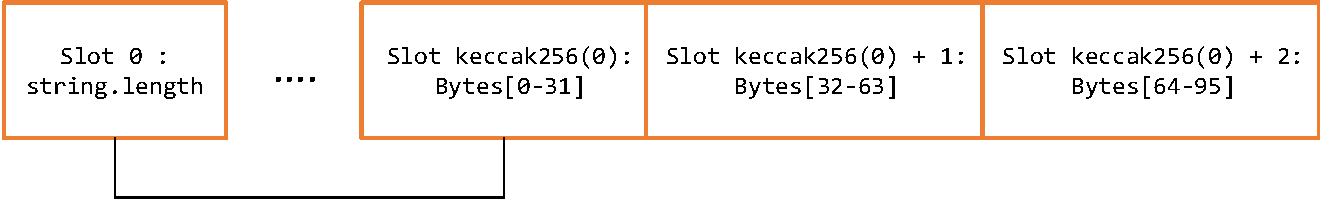
\includegraphics[width=9cm]{figs/Storage.pdf}}
\caption{Layout of dynamic arrays in SC storage.}
\label{fig:arrays}
\end{figure}

Static types are stored consecutively in storage, occupying one or more slots, depending on their size. Due to their unpredictable size, dynamic data types cannot adhere to the same principles. Regarding dynamic arrays, their starting position is determined using the keccack hash function. At first, a storage slot that holds its length is initialized at some position, p, and then the array’s data are stored starting at position keccack(p), as shown in Fig.~\ref{fig:arrays}. Solidity’s strings and bytes are special dynamic arrays with a somewhat nuanced behavior. As long as they are less than 31 bytes, their data are stored in the same position, p, as their length. When this threshold is exceeded the rules of dynamic arrays apply.

\subsection{Storing Data in Event-logs}\label{subsection:}
Every transaction receipt in the Ethereum blockchain contains log entries (logs), which are indexable checkpoints in EVM code execution  \citep{wood_2014}. In the context of Solidity, EVM’s logging operations are facilitated by the use of events. When emitting an event inside a SC, its parameters are stored in logs. Mostly, they are used as a way of triggering a change in an application’s front end or returning a value from a function  \citep{consensys}. Nonetheless, they can also be used as a means of cheaper data storage. It is noteworthy that the data stored in logs are not accessible from SCs, consequently logs cannot replace storage.

\begin{table}[htbp]
\caption{Generalized cost model for different types of events. Gas costs were populated according to the logging operations $G_{\mathrm{logdata}}$ and  $G_{\mathrm{logtopic}}$ which are presented in table \ref{table:operations_cost}.}
\label{table:event_cost}
\resizebox{\textwidth}{!}{%
\begin{tabular}{@{}cccc@{}}
\toprule
 & \textbf{Indexed} & \textbf{Non-Indexed} & \textbf{Anonymous} \\ \midrule
\textbf{Topic{[}0{]}} & Signature Hash (375 gas) & Signature Hash (375 gas) & - \\
\textbf{Topic{[}1{]}} & Indexed Parameter (375 gas) & - & - \\
\textbf{Log Data} & Data (data.len*8 gas) & Data (data.len*8 gas) & Data (data.len*8 gas) \\ \bottomrule
\end{tabular}%
}
\end{table}

In general, logs consist of the caller’s address, a series of topics and some bytes of data. A BF is utilized to efficiently search for certain logs, based on the caller’s address and topics. When declaring an event, one can specify the keyword indexed for up to three parameters. This will result in a respective number of topics in the produced logs, allowing for a more efficient query, known as filtering. By default, both indexed and non-indexed events store the hash of their signature, which is comprised of information that can later be found in the contract’s ABI and used for filtering, as the first topic. A developer can avoid this by declaring the event as anonymous, making it less expensive to call (Table~\ref{table:event_cost}) but more difficult to retrieve.

\subsection{Storing Data in Transaction Payload}\label{subsection:}
In Ethereum there are two types of transactions, those leading to message calls and those which result in contract creation. A message call is the act of passing some value and arbitrary binary data between accounts, either of which can be null. If the target account is a Contract Account (CA), its code is executed with the data part of the message, also termed transaction payload, as input. It is notable that transactions between Externally Owned Accounts (EOAs), may as well contain non-empty payload, transfer no value or even be self-transactions, i.e., the transaction's target is the sender.

As a rule, all transactions, including any payload, are permanently stored in the blockchain. Hence, sending data through a transaction turns out to be an alternative storage method. Considering that 16 gas is charged for every non-zero byte of a transaction’s data and 4 gas for every zero byte, this technique seems appealing. Though, one cannot ignore the fact that such data are not available inside the SC and retrieving them requires storing the corresponding transaction hash, probably in an external database as proposed by Xie et al. \citep{xie_2017}. Apart from that, a transaction payload is, at its core, a hex byte array, which implies that for more complex data types, additional logic should be implemented on the client side.

\begin{figure}[htbp]
\centerline{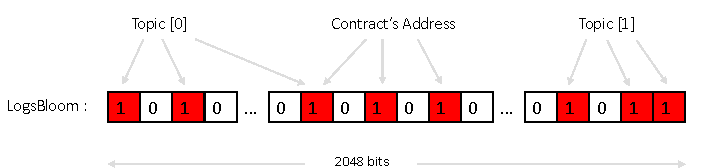
\includegraphics[width=\textwidth]{figs/bloom.pdf}}
\caption{Example of the bloom bits set by an event.}
\label{fig: bloom}
\end{figure}

\subsection{Storing Data in Unused Function Parameters}\label{subsection:}
With this term we refer to input data that are passed as function parameters but are no further used within function’s body, as seen in Fig.~\ref{fig:un}. This process is slightly more expensive than the previous one, as it is mandatory for function arguments to be ABI encoded, resulting in a longer payload array. However, it provides better functionality since the underlying tools for encoding and decoding such data are already developed  \citep{web3}, allowing the use of complex data types.

\begin{figure}[htbp]
\setlength{\fboxsep}{5pt}%
\setlength{\fboxrule}{0.05pt}%
\centerline{\fbox{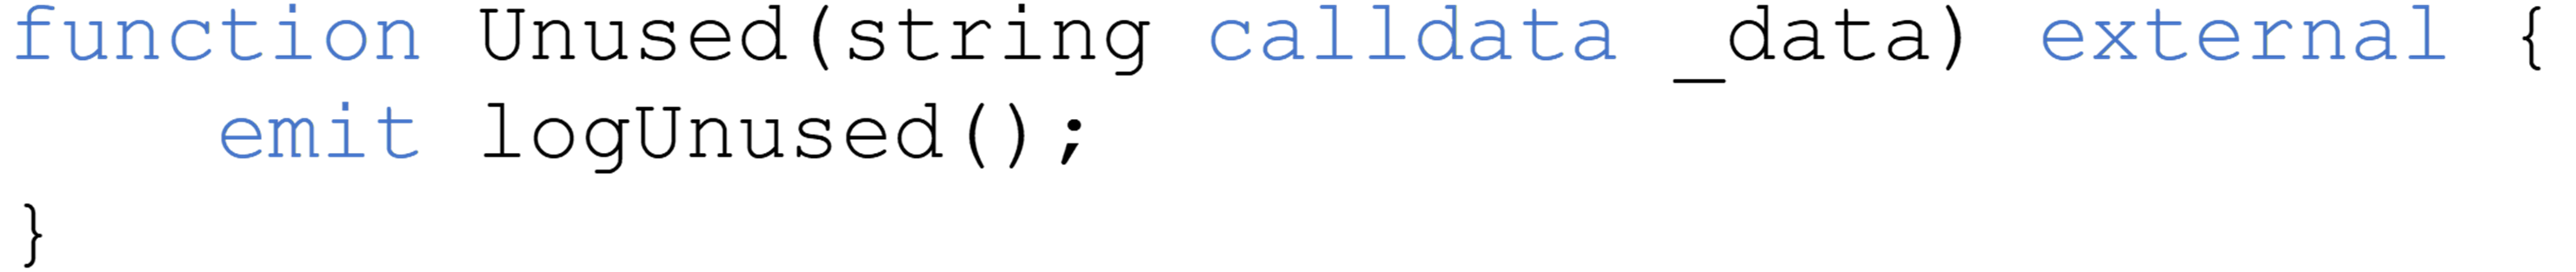
\includegraphics[width=12cm]{figs/code.png}}}
\caption{Basic example of the unused function parameters method.}
\label{fig:un}
\end{figure}

Moreover, this method includes a function call and therefore permits the execution of additional logic during the same transaction, as opposed to the aforementioned method. For instance, an event could be emitted inside the function, providing a way of future-tracking the respective transaction and retrieving its data, eliminating the need for storing the transaction hash externally.

\subsection{Retrieving logs}\label{subsection:}
In Ethereum log retrieval is accomplished with a specialized BF  \citep{wood_2014}. A BF  \citep{broder_2004} is a space-efficient probabilistic data structure used to quickly check whether an element is part of a set. 

A BF is represented by an array of m bits $\{b_1, b_2,…, b_m\}$ all initialized to zero. An element is inserted into the BF as follows. Its value is hashed k times with k independent hash functions $\{h_1, h_2,.., h_k\}$. Each time, based on the resulting hash and a mathematical formula, a bit of the BF is set to one. To determine if an element is present in the set, the same process is repeated. If all the k corresponding bits are 1s, then the element might be in the set. Otherwise, it is certainly not part of the set. In other words, a BF may return false-positives but never false negatives.

In Ethereum, every block includes a BF of 2048 bits. Each event emitted by the block’s transactions generates a log entry that sets at least three bits of the BF based on the contract’s address, and another three bits for every topic (if any), as shown in Fig.~\ref{fig: bloom}. The bits are determined by calculating the modulo 2048 of each of the first three pairs of bytes in the Keccak-256 hash of the input, where input is the contract’s address or a topic  \citep{wood_2014}.

When it comes to retrieving a specific log, each block’s BF needs to be inspected. If any of the bits that correspond to the topics or the contract’s address is zero, then, the log indeed isn’t part of the block. If all corresponding bits are set, the logs of the block are loaded and inspected individually. In case of a false positive the next block needs to be inspected.
To sum up, using BFs is much more efficient than a conventional search, but be that as it may, it is still time consuming because false positives are common and lead to additional retrievals to check if the log is the desired one. As expected, our findings (Section \ref{subsec:retrieve}) confirm that limiting the block filtering range can substantially reduce the retrieval latency.

\section{Hybrid Schemes}\label{sec:}
The Ethereum blockchain, while effective for executing code and processing data in a decentralized manner, it is not optimized for storing large volumes of data due to high costs \hl{and low space}. Consequently, in scenarios where decentralized applications must handle a lot of data, a direct on-chain storage approach isn't viable.

\begin{figure}[htbp]
\centerline{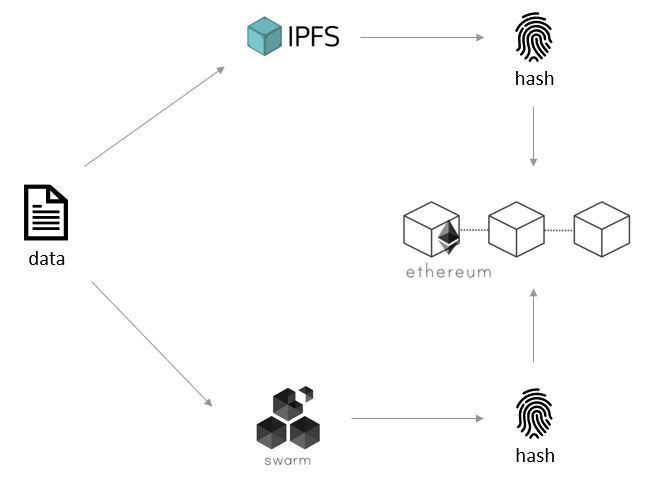
\includegraphics[width=12cm]{figs/hybrid.png}}
\caption{Hybrid architecture overview.}
\label{fig: hybrid}
\end{figure}

Distributed file systems like IPFS and Swarm can be integrated with blockchain networks like Ethereum to overcome limitations related to data storage, providing a scalable and efficient solution for fully decentralized applications. With that being said, most blockchain-based applications with high storage requirements would need to consider an on-chain/off-chain hybrid architecture.

Data storage in hybrid schemes follows a two-step approach as shown in fig. \ref{fig: hybrid}:
\begin{enumerate}
\item Data is stored in a distributed file system (IPFS or Swarm) and a unique identifier is generated for it.
\item The unique identifier is stored in the Ethereum blockchain.
\end{enumerate}

% To summarize, coupling a blockchain with a distributed file system allows for decentralized and secure storage and retrieval of data.
The immutable nature of the blockchain provides a tamper-proof way of storing the identifiers. Besides that, blockchain technology provides a built-in mechanism for timestamping (each block contains a timestamp). This can be leveraged to create provable timestamps for data stored off-chain. In conjunction with the characteristics of self-verification and authenticity that distributed file systems offer through content addressing, data integrity of such schemes is guaranteed.

When it comes to storing the identifiers in Ethereum, any of the methods that we described in the previous paragraphs can be adopted. Storing them in SC storage is the most straightforward option. On the other hand, alternatives like the event-logs, the transaction payload or the unused function arguments are far less expensive. In addition, the retrieval latency of each approach must be considered as well. Both aspects are examined and discussed in detail in the next chapter, which will hopefully enable developers to make a more informed choice.

For data retrieval, the process is simple. The DApp retrieves the identifier from the blockchain and then uses it to retrieve the actual data from the respective distributed file system.

\cleardoublepage
\chapter{Experimental Evaluation}\label{chapter:experiments}
In this section we describe the experimental environment and provide details about the criteria we chose to focus on, and the steps followed in our experiments. Besides that, we discuss the corresponding results. The project's source code and other supplementary material are available on GitHub\footnote{\url{https://github.com/perikost/ExploringEthereum}}.

Before proceeding further, we should mention an important detail concerning the data we used during our experiments. Solidity uses UTF8 encoding, according to which common ASCII characters are represented by a single byte. Additionally, generating random fixed-length character sequences is simple and all the methods we examined support this format. So, to evaluate the cost of storage in Ethereum, for each test case, we recorded 15 measurements regarding various string sizes equally spread across the range of 1B-16KB. However, for those cases that exhibited consistent behavior we present only part of our measurements.

\section{Experimental Setup}\label{sec:}
\subsection{Local experiments}\label{sec:}
We conducted our experiments on a machine with i7-8700 CPU, 64GB RAM, 2TB SSD running Ubuntu 20.04. All SCs were written and compiled in Solidity 0.8.12 with the optimizer disabled and were deployed on Ropsten Testnet. Geth version 1.10.16 was used as an Ethereum client. For IPFS and Swarm, IPFS-client version 0.7.0 and Swarm Bee Client version 0.5.0 were used, respectively.
\subsection{Remote Experiments}\label{sec:}
Grid5000...
\section{Criteria}\label{sec:}
For evaluating the sustainability of using Ethereum as a stand-alone data store, we emphasized on the associated gas cost. In this regard, we thoroughly examined the most common storage methods, the SC storage, and the event-logs. Considering these as reference points, we explored alternatives and cost-wise compared the resulting gas costs. In addition, the implementation complexity of each approach was considered. Our findings are summarized in Table~\ref{table:overall}. On the other hand, the respective costs of the hybrid schemes are presented in Table~\ref{tab:hash_cost}. Among others, the results confirm that the use of SC storage incurs costs that are orders of magnitude larger than the alternative data stores we examined.

Except for being monetarily viable, DApps need to perform adequately when it comes to retrieving data. That being said, we measured the retrieval time in all the above scenarios. For IPFS and Swarm, both upload and retrieval performances were taken into account, aiming to a better overall comparison.
\section{Experiments - Storing Data in Ethereum}\label{sec:}
\subsection{SC Storage}\label{subsection:}
\begin{figure}[htbp]
    \begin{subfigure}{\linewidth}
        \centerline{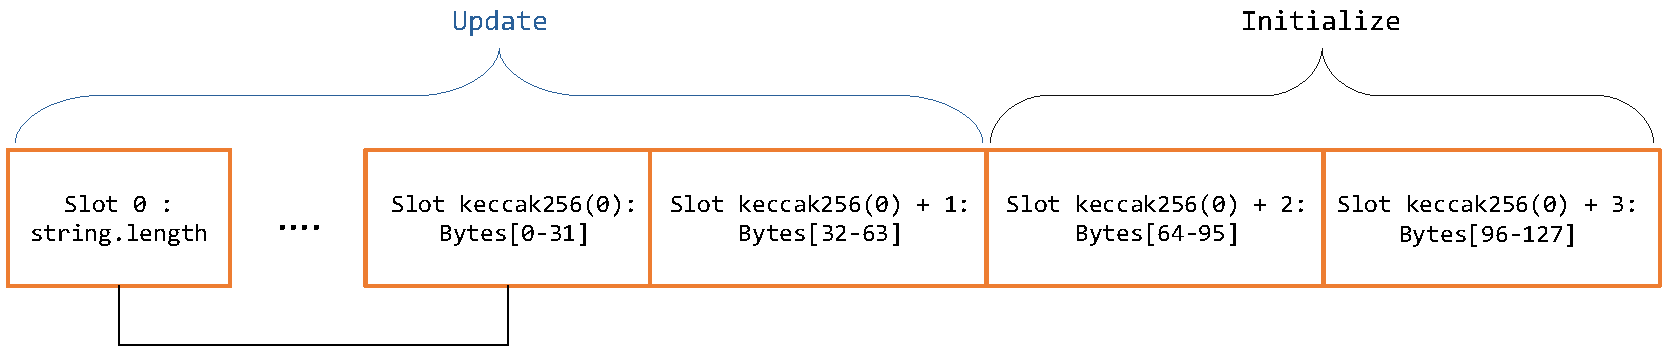
\includegraphics[width=9cm]{figs/Storage1.pdf}}
        \caption{}
        \label{fig:arrays_1}
    \end{subfigure}
    \begin{subfigure}{\linewidth}
        \centerline{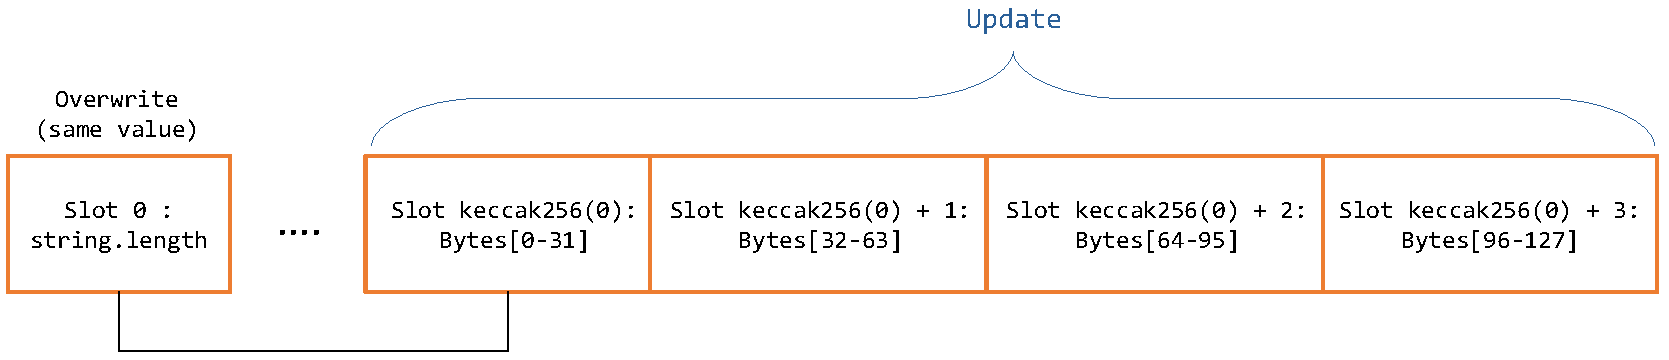
\includegraphics[width=9cm]{figs/Storage2.pdf}}
        \caption{}
        \label{fig:arrays_2}
    \end{subfigure}
    \caption{Slots that must updated or initialized when overwriting a string with (a) a longer (b) a new one of the same size.}
\end{figure}

In order to perform this experiment, we designed a simple SC with the following elements: a public string variable to store our data, a function to modify this string and another one to reset it. In total, we tested three of the most common scenarios.

\begin{itemize}[topsep=0pt, itemsep=0pt]
  \item Storing data after resetting the variable (clean storage).
  \item Updating the variable to a longer string (double the size), Fig.~\ref{fig:arrays_1}.
  \item Updating the variable to a new string (same size), Fig.~\ref{fig:arrays_2}.
\end{itemize}

The baseline of 21000 gas for every transaction and the gas paid for its payload are equal in all three cases. So, the number of slots that must be overwritten or initialized during each test case mostly accounts for the difference in the respective costs depicted in Fig.~\ref{fig:store1} and Fig.~\ref{fig:store2}, which was included to present the costs for small data. For data less than 32 bytes, as discussed in subsection~\ref{sec:storage}, one slot is adequate. Otherwise, \(\ceil*{x/32}\) slots for storing the data and one for storing the string's size \(x\), are required. In the case of clean storage, all slots must be initialized, costing \(20000*num\_slots\) gas. When updating a string with a new one of the same size, 5000 gas is deducted for each of the \(\ceil*{x/32}\) slots. Note that the slot holding the string’s length is not updated, as the string’s size does not change. In fact it is overwritten with the same value, which is termed as a \emph{``no-op''} and is charged equally to an SLOAD operation. The second case is a combination of the others and so is the cost calculation method. Some slots must be initialized, and others need to be updated, costing 20000 and 5000 each.

\begin{figure}[htbp]
\centerline{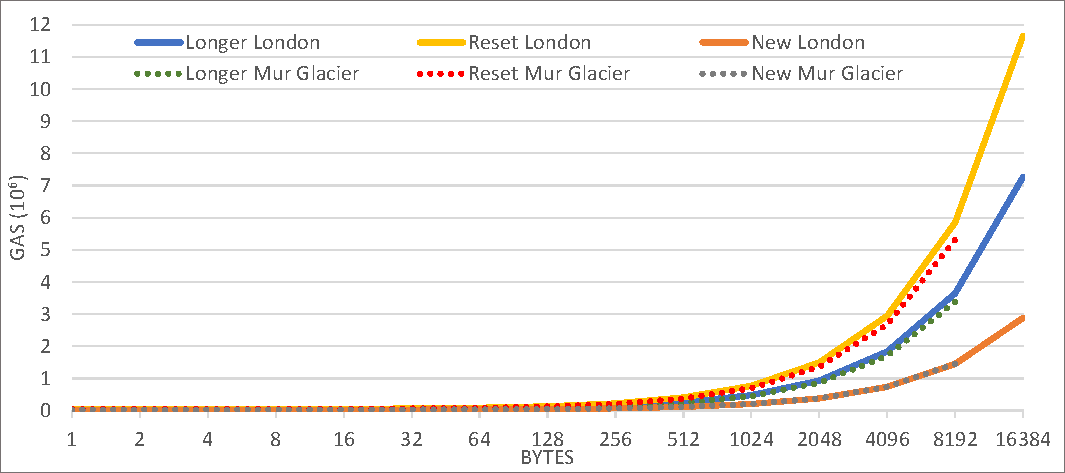
\includegraphics[width=9cm]{figs/store1.pdf}}
\caption{SC storage cost diagram.}
\label{fig:store1}
\end{figure}

\begin{figure}[htbp]
\centerline{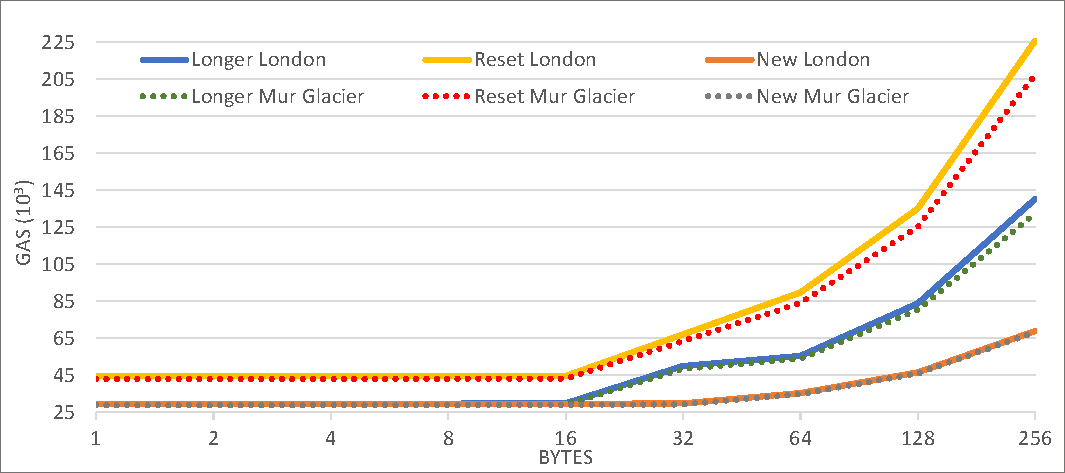
\includegraphics[width=9cm]{figs/store2.pdf}}
\caption{Zoomed in view of the diagram in Fig.~\ref{fig:store1}.}
\label{fig:store2}
\end{figure}

Up to this point, we discussed gas consumption based on the EIPs introduced prior to (including) Muir Glacier. EIP-2929  \citep{buterin_eip_2929}, included in Berlin fork, reforms SLOAD and SSTORE gas metering. We only present the changes that were found to affect our test cases. As reference, the corresponding Geth’s implementation was used  \citep{ethereum_2022}.

\vspace{0.2cm}
\noindent
\textsc{sload} cost modification:
   \begin{itemize}[topsep=0pt, itemsep=0pt]
     \item  \textsc{warm\_sload}: charge 100 gas if slot has already been accessed in current execution context.
     \item  \textsc{cold\_sload}: charge 2100 gas if slot has not been accessed in current execution context.
   \end{itemize}
   
\vspace{0.2cm}
\noindent
 \textsc{sstore} cost modification:
   \begin{itemize}[topsep=0pt, itemsep=0pt]
     \item  Initialize a slot:
     \begin{itemize}[topsep=0pt, itemsep=0pt]
        \item If slot is not already accessed: charge \textsc{cold\_sload} + \textsc{sstore} = 2100 + 20000 = 22100
        \item If slot is already accessed: charge \textsc{sstore} = 20000
     \end{itemize}
   \end{itemize}
   
   \begin{itemize}[topsep=0pt, itemsep=0pt]
     \item  Update a slot: 
     \begin{itemize}[topsep=0pt, itemsep=0pt]
        \item If slot is not already accessed: charge \textsc{cold\_sload} + \textsc{(sstore\_reset - cold\_sload)} = 5000
        \item If slot is already accessed: charge \textsc{(sstore\_reset - cold\_sload)} = 5000 – 2100 = 2900
     \end{itemize}
   \end{itemize}
   
   \begin{itemize}[topsep=0pt, itemsep=0pt]
     \item  Overwriting a slot with the same value (no-op):
     \begin{itemize}[topsep=0pt, itemsep=0pt]
        \item If slot is not already accessed: charge \textsc{(cold\_sload + warm\_sload)} = 2100 + 100 = 2200
        \item If slot is already accessed: charge \textsc{warm\_sload} = 100 
     \end{itemize}
   \end{itemize}
   
Considering the altered cost model, we re-executed all test cases to examine Ethereum’s actual behavior after the Berlin hard fork. In order to be up-to-date, we also repeated our study when the London hard fork was implemented. Gas consumption related to the SSTORE and SLOAD operations was not altered by any of the included EIPs. However, EIP-1559 specifies a transaction pricing mechanism that temporarily raises the block’s gas limit when congestion occurs. This enabled us to store up to 16KBs in contrast to the 12KBs that we managed to store in previous experiments. In Fig.~\ref{fig:store1} we present our most recent results, since they reflect the impact that both hard forks induced.

\begin{table}[htbp]
\caption{Impact of the Optional Access List}
\label{table:access_list}
\resizebox{9cm}{!}{%
\begin{tabular}{@{}lll@{}}
\toprule
 & \textbf{No access list} & \textbf{Access list}  \\ \midrule
\textbf{Account} & \begin{tabular}[c]{@{}l@{}}2600 for first access + \\ 100 for each subsequent access\end{tabular} & \begin{tabular}[c]{@{}l@{}}2400 to be included in the AL + \\ 100 for each access\end{tabular} \\
\textbf{SLOAD} & \begin{tabular}[c]{@{}l@{}}2100 for first access + \\ 100 for each subsequent access\end{tabular} & \begin{tabular}[c]{@{}l@{}}1900 to be included in the AL + \\ 100 for each access\end{tabular}
\\
\textbf{SSTORE} & \begin{tabular}[c]{@{}l@{}}22100 for each initialization\end{tabular} & \begin{tabular}[c]{@{}l@{}}1900 to be included in the AL + \\ 20000 for each initialization\end{tabular}
\\
\textbf{SSTORE} & \begin{tabular}[c]{@{}l@{}}5000 for each update\end{tabular} & \begin{tabular}[c]{@{}l@{}}1900 to be included in the AL + \\ 2900 for each update\end{tabular}
\\
\textbf{SSTORE} & \begin{tabular}[c]{@{}l@{}}2200 for each each update (same value)\end{tabular} & \begin{tabular}[c]{@{}l@{}}1900 to be included in the AL + \\ 100 for each update (same value)\end{tabular}
\\* \bottomrule

\end{tabular}%
}
\end{table}

Overall, all transactions after EIP- 2929 had a higher cost, especially those regarding our first test case, in which, every slot had to be initialized imposing an overhead of 2100 gas. Regarding the third test case, all transactions executed after the fork proved to cost 600 more. By debugging those, we discovered that this difference is caused by the SLOAD gas metering modification. Basically, when updating a string, the slot that holds the string’s length is accessed twice; once to determine the string’s length (SLOAD) and a second time to update it to the new length (SSTORE). The SLOAD operation is considered a COLD\_SLOAD and costs 2100 gas. The SSTORE on the currently \emph{``warm''} slot is considered a \emph{``no-op''} since the length of the string remains the same and costs 100 gas. Before EIP-2929 took effect, these operations were charged 800 each.

\begin{figure}[htbp]
\centerline{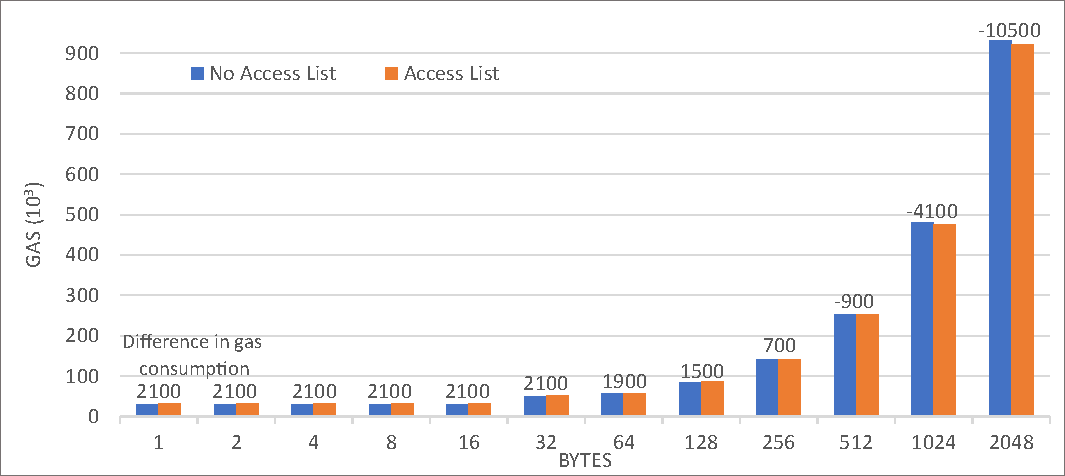
\includegraphics[width=9cm]{figs/access_list.pdf}}
\caption{SC storage cost diagram (optional AL).}
\label{fig:access_list}
\end{figure}

Besides EIP-2929, EIP-2930 was also included in the Berlin hard fork. EIP-2930  \citep{buterin_eip_2930} adds a new transaction type and introduces the notion of an optional AL, a list of addresses and storage keys that the transaction plans to access. This essentially enables a user to “warm-up” the accounts and storage slots they plan to access, at a discounted cost. The following equation gives the intrinsic cost of the new transaction type:

\begin{flushleft}
\centering
$ 21000 + 16 * \textsc{non\_zero\_bytes} + 4 * \textsc{zero\_bytes} + 1900 * \textsc{storage\_key\_count } + 2400 * \textsc{address\_count}$
\end{flushleft}

% \begin{flushleft}
% \centering
% $\textsc <cidv1> ::= <multibase><multicodec-version><multicodec-content-type><multihash>$
% \end{flushleft}

% \[
% 21000 + 16 * \textsc{non\_zero\_bytes} +
% 4 * \textsc{zero\_bytes} +
% 1900 * \textsc{storage\_key\_count } +
% 2400 * \textsc{address\_count}
% \]

\vspace{0.2cm}

All the accounts and storage slots specified in the AL are considered “warmed up” and consequently SLOAD, *CALL, BALANCE, EXT* operations on them are charged as if they were already accessed, in accordance with EIP-2929. Table~\ref{table:access_list} is a simplified representation of the access-cost when an AL is or is not utilized.

Based on Table~\ref{table:access_list} one would assume that declaring an AL is a better option, at all times, as 100 gas would be saved for every account/storage access and 200 gas for every SSTORE operation. However, that is not the case. If storage keys of the targeted contract are specified in an AL, the targeted contract account must be included as well, imposing an overhead of 2400 gas. 

\begin{figure}[htbp]
\centerline{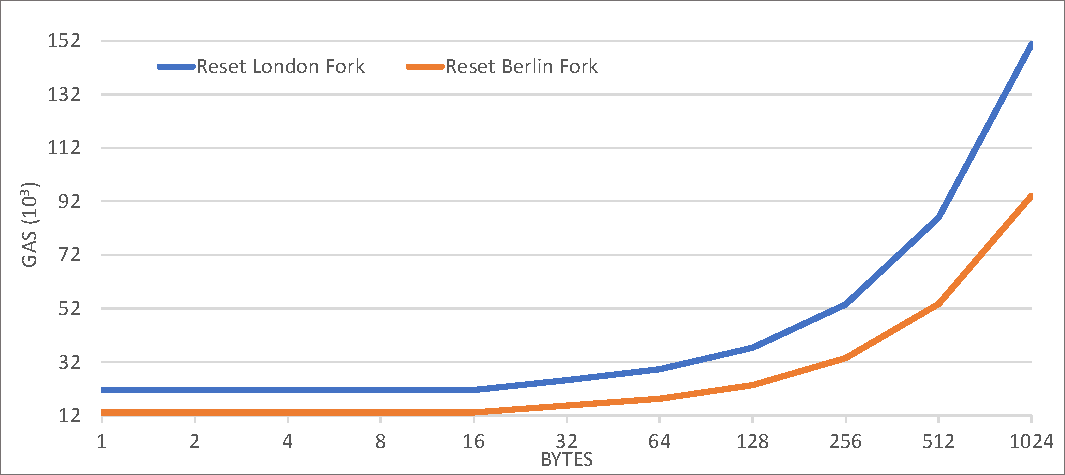
\includegraphics[width=9cm]{figs/reset.pdf}}
\caption{Cost of clearing SC storage.}
\label{fig:reset}
\end{figure}

The behavior described above is depicted in Fig.~\ref{fig:access_list}. When the string’s size is under 352 bytes, using an AL is more expensive due to the gas paid for including the contract’s address. On the contrary, storing a string longer than 352 bytes is more cost-efficient if an AL is declared. In brief, the 2400 overhead is countered by the 12 or more SSTORE operations that access each of the storage slots that contain the string's data and the SLOAD operation required to determine the string's length, which are charged at a discounted rate, i.e., 200 and 100 less gas respectively.

As a general guide, one should opt in for the use of ALs, but refrain from specifying storage slots of the targeted contract account. Yet, if the main contract interacts with other contracts, which then access their storage, specifying their addresses (but not tx.to) and storage keys in an AL is less expensive than not using an AL.

Handling the data of a DApp involves data storage, retrieval and deletion. In Ethereum, SC storage is considered a valuable resource and therefore a gas refund is given when data is erased.

In Fig.~\ref{fig:reset}, we present the overall cost associated with clearing the slots occupied by a string’s data. Considering that clearing a slot entails updating its value from non-zero to zero, the actual execution cost is comparable to that of updating a string to a new one (see Fig.~\ref{fig:arrays_2}), except that in this case the string's length is also updated; 5000 gas is charged for every SSTORE operation on the slots that the string occupies. Though, the refund granted for these operations contributes to a lower overall transaction cost.

London hard fork introduced EIP-3529  \citep{buterin_eip_3529} which modified the refund mechanism. Prior to this, emptying a slot was rewarded with 15000 gas and the total refund was capped at 50\% of the transaction’s gas used. In the London fork implementation both the reward and the refund were reduced to 4800 gas and 20\%, respectively. Fig.~\ref{fig:reset} demonstrates the impact that this modification has on the cost related to deleting a string. All transactions incurred an increase of approximately 38\% in gas usage.

\subsection{Event-logs}\label{subsection:}

Prior to any further analysis, we ought to mention that in preliminary experiments, counters were used as identifiers (ids) for the events, as illustrated in Table~\ref{table:event}. However, the use of counters entails the execution of an SLOAD operation, which gets their values in order to pass them as parameters to the events and also an SLOAD and SSTORE operation for incrementing them, imposing an overhead of 6600 gas in every transaction. Considering this, in our recent experiments, we decided to pass the ids as arguments. Hence, the results presented in this work are rather indicative of the effect that emitting an event has on gas consumption, as the need for extra contract logic was eliminated.

As we can observe in Fig.~\ref{fig:logs} the resulting costs from calling each event, exhibit relatively small divergence. Through  \citep{wood_2014} we know that each topic costs 375 gas. Respectively, there is a charge of 8 gas for each byte of data recorded in the data field of the logs. Thereby, the number of topics generated by the event call in each of the cases we examined, as well as the amount of data recorded in the log data field, are key factors in the cost variance between them. These are determined by the way the events are declared, as shown in Table~\ref{table:event}. If the id is indexed it is placed in the topics array along with the event’s signature hash, otherwise it is ABI encoded into the data field of the log. Additionally, since the input data are identical in all the events and the contract's code is immutable by default, the constant gap maintained by the four graphs is justified.

\begin{table*}[]
\caption{Structure of events and logs included in the experiments}
\centering
\label{table:event}
\resizebox{15cm}{!}{%
\begin{tabular}{@{}ccccc@{}}
\toprule
 & \textbf{Indexed} & \textbf{Non-Indexed} & \textbf{Anonymous Indexed} & \textbf{Anonymous} \\ \midrule
\textbf{Declaration} & \begin{tabular}[c]{@{}c@{}}event\_name(uint indexed id, \\ string data)\end{tabular} & \begin{tabular}[c]{@{}c@{}}event\_name(uint id, \\ string data)\end{tabular} & \begin{tabular}[c]{@{}c@{}}event\_name(uint indexed id, \\ string data) anonymous\end{tabular} & \begin{tabular}[c]{@{}c@{}}event\_name(uint id, \\ string data) anonymous\end{tabular} \\
\textbf{Topic{[}0{]}} & keccak(event\_signature) & keccak(event\_signature) & - & -\\
\textbf{Topic{[}1{]}} & abi\_encode(id) & - & abi\_encode(id) & - \\
\textbf{Log Data} & abi\_encode(data) & abi\_encode(id, data) & abi\_encode(data) & abi\_encode(id, data) \\ \bottomrule
\end{tabular}%
}
\end{table*}

It should be noted that because log data is ABI encoded, even a uint8 occupies 32B and is charged \( 8*32 = 256 \) gas. For this reason, converting a non-indexed parameter to an indexed does not impose much of an overhead. In fact, it is negligible since the opcodes that are executed to determine the function to be called, might result in the indexed event being less expensive. That is the case for the anonymous events, as indicated in Fig.~\ref{fig:logs}.

Finally, even though anonymous events are the least expensive option, they should be used frugally. The fact that they don’t register their signature as a topic, prohibits them from being uniquely referenced, perplexing their retrieval. Including indexed parameters to such events can assist with that.

% Finally, it is apparent that the use of SC storage incurs costs that are orders of magnitude larger than the currently discussed alternative.

\begin{figure}[htbp]
\centerline{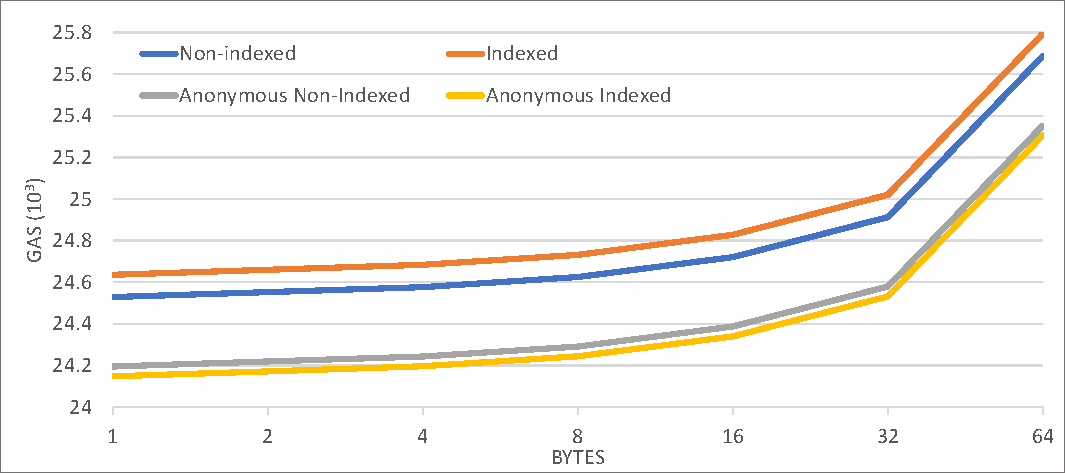
\includegraphics[width=9cm]{figs/logs_1.pdf}}
\caption{Event-logs storage cost diagram.}
\label{fig:logs}
\end{figure}

\subsection{Transaction Payload}\label{subsection:}
The first step of this experiment was to encode the data in hex format. Then, we included the resulting hex byte array in the data field of a transaction object, signed it and sent it. Note that no ether was transferred during any of the transactions. We tried two different ways of implementing this method:

\begin{itemize}[topsep=0pt, itemsep=0pt]
  \item Sending the transaction between EOAs
  \item Sending the transaction from an EOA to a CA
\end{itemize}

As expected, the measurements confirm that the use of transactions as a data store is the most cost-efficient solution of all when data is sent between EOAs. As a matter of fact, this can be considered the minimum cost for storing data in Ethereum. That is, because the fee paid for a transaction’s payload is essentially included in every available option, e.g., for executing a transaction with some data as input, these data must first be sent as payload to the contract.

For the second case we tested, a fallback function in the targeted SC is required, otherwise the transactions will fail. In short, fallback is a special function that gets executed if none of the function selectors match the first four bytes of the transaction payload, or if the latter is empty and no Receive Ether function is defined. Additionally, it cannot have parameters nor return anything. The body of the fallback could either be empty or include function logic. In any case, if arbitrary hex-encoded data is included in the payload of a transaction that is targeted to a SC, the fallback will be executed (no function selector will be matched) and the data will be permanently saved in the blockchain, as part of the transaction. Implementing an empty fallback entails that the transaction hash must be saved externally. On the contrary, emitting an event inside the fallback allows the user to obtain the transaction hash from the resulting logs and retrieve the data from the recorded transaction.

\begin{figure}[htbp]
\centerline{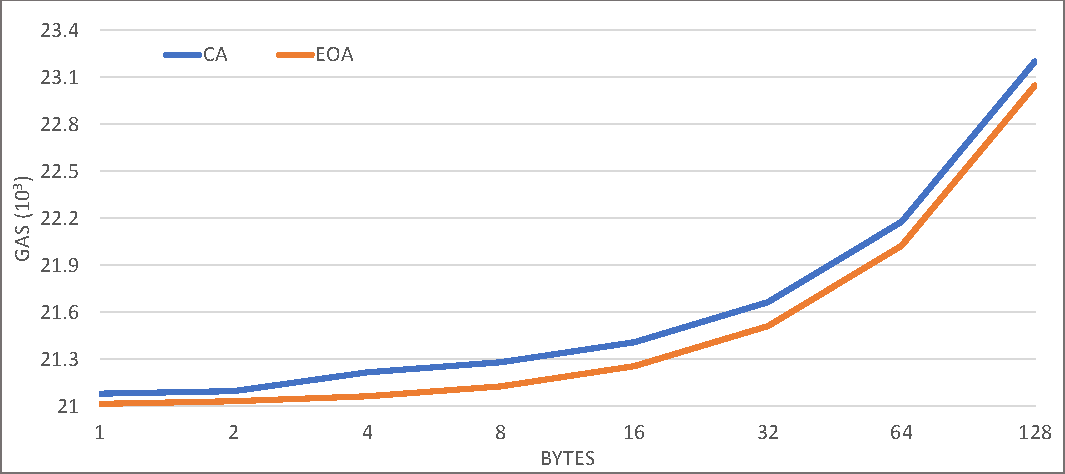
\includegraphics[width=9cm]{figs/tx.pdf}}
\caption{Transaction payload storage cost diagram.}
\label{fig:tx}
\end{figure}

Based on Fig.~\ref{fig:tx}, we are able to compare the cost of saving data in a transaction payload that is sent to an EOA or a CA, respectively. Regarding the latter scenario, the SC implements an empty fallback function. The difference between the amount of gas spent in each test case stems from the fact that in the second one some contract code needs to be executed. By inspecting the bytecode of the corresponding contract, we managed to further analyze this difference. After verifying that no ether was sent with the transaction, a series of opcodes is executed to check if the payload is less than four bytes. If that is true, EVM jumps to fallback’s execution. The accumulated cost resulting from the EVM execution, up to that point, is 65 gas greater than that of test Case 1. If the aforementioned condition is false, the first four bytes of the payload are loaded and processed, costing 12 gas, and they are compared against every function selector of our contract’s three functions. Eventually, no match is found and the execution jumps to the fallback function, which costs 10 gas. The code blocks in which the comparisons are conducted consist of the opcodes \textsc{\{dup1, push4, eq, push2, *jumpi\}}, which altogether cost 22 gas. Taking into account that no match will be found, all comparisons are executed, costing 66. In total, the cost for storing \(data\geqslant 4\) bytes in a transaction by exploiting the fallback function, is 153 gas greater than the other test case.


By inspecting the execution of the contract at bytecode level we managed to verify what to our knowledge was first reported, but not explained, in \citep{chen_2018}. Simply put, function selectors, which are comprised of the first four bytes of the Keccak-256 hash of the function's signature and therefore depend on function names and parameter types, are compared to the first four bytes of a transaction’s payload in hex-ascending order. Hence, frequently used functions should be named in an appropriate manner to avoid numerous comparisons, i.e., save gas. Moreover, we believe it is necessary to point out that for a contract with a large number of functions, Solidity optimizes the comparison flow by performing a pre-comparison to check whether the given function selector is or is not above a certain threshold.

As already mentioned, an event could be emitted inside the fallback function to avoid saving the transaction hash off-chain. Similarly to the experiments in~\ref{par:event_exp}, the event should include an id parameter so that the data can be identified upon retrieval. This was achieved in two ways: i) increasing a counter in every call ii) reserving some bytes of the transaction data (e.g., the first 32bytes) to hold the id. The latter is generic since values other than integers can be used, but requires additional logic, both on-chain and off-chain, to separate or concatenate the data and the id. In addition, eschewing the use of a counter significantly reduces the gas consumption, as depicted in Fig.~\ref{fig:fallback}. In fact, since the cost of the log operation is identical in both cases, the difference in the cost depends solely on the need of updating the counter, which involves two SLOAD and one SSTORE operations.

\begin{figure}[htbp]
\centerline{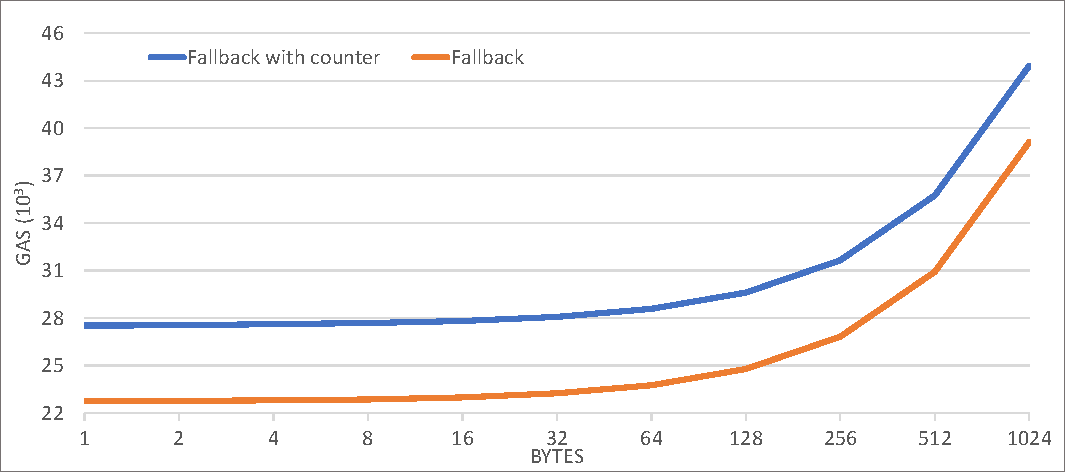
\includegraphics[width=9cm]{figs/fallback.pdf}}
\caption{Cost of emitting an event inside the fallback function.}
\label{fig:fallback}
\end{figure}

\subsection{Unused Function Parameters}\label{subsection:}
This experiment was performed to examine the cost of storing data in a transaction’s payload while exploiting Solidity’s built-in ABI interface.
Such a scheme overcomes the restriction imposed by the previous method as it facilitates the management of all the data types that Solidity supports, without the need of additional client logic. 

% we used a function with a single parameter that was no further processed.
% \hl{We also decided to improve the functionality of this method by emitting an event, with just one indexed parameter, inside the function in order to track the hash of the transaction at a later point}.
In order to examine this approach, we declared a function with two parameters; one to hold the data and another one to hold an identifier. The former was no further processed, while the latter was passed to an event. Emitting an event inside the function enabled us to obtain the transaction hash from the resulting logs and retrieve the ABI encoded data from the recorded transaction. In contrast to the utilization of a fallback function, which cannot accept any arguments, the id of the event is passed as a function argument eliminating the need for additional contract logic.

To evaluate the recorded costs, we used the case of indexed events as a reference point. It is obvious from Fig.~\ref{fig:unused} that as input data grow in size, the current approach gets even cheaper than the other. The fact that in this case, no data are recorded in the data part of the produced log, accounts for the difference.

\begin{figure}[htbp]
\centerline{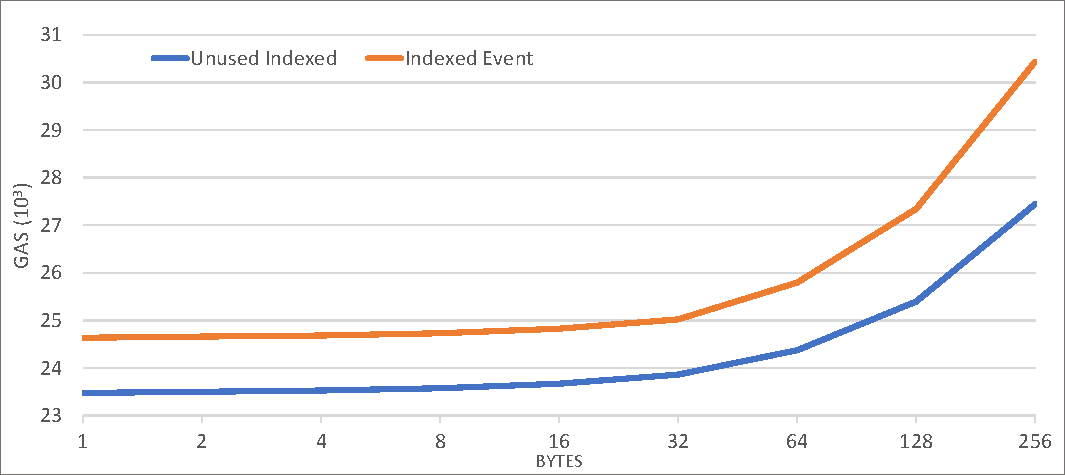
\includegraphics[width=9cm]{figs/unused.pdf}}
\caption{Unused function parameter and event-logs storage cost diagram.}
\label{fig:unused}
\end{figure}

As we already mentioned, the fact that non-indexed parameters are ABI encoded into the log data leads to long log arrays. So, in a scenario in which more unused parameters are utilized, the current approach is even less expensive. To confirm this, we conducted a complementary experiment, locally in Ganache. A contract with two functions carrying seven parameters each was deployed. Function 1 emitted an event with all parameters as input, whereas Function 2 emitted an event with just the first parameter. After executing both functions with the same arguments, we concluded that the utilization of unused function parameters can be quite effective, as Function 2 cost nearly 7000 less gas.

At this point, we would like to discuss some possible drawbacks regarding this alternative storage method. First, by testing we discovered that Solidity imposes a restriction on the number of parameters a function can bear (around sixteen). If this threshold is exceeded, a \emph{``stack too deep''} error is thrown. Additionally, defining a function with unused function parameters causes a warning at compilation. Thus, it might be disallowed in future Solidity versions.

\section{Experiments - Data Retrieval in Ethereum}\label{sec:}
In this subsection, based on our experimental measurements, we present an overall comparison of the time needed to retrieve data from the Ethereum blockchain. Each measurement refers to the retrieval time of the data that were stored during the previous experiments. We noticed that the results were quite similar for the different data sizes (1B – 16KB), so, in Table~\ref{tab:retrieve} we recorded the average of these results. Also, we should mention that retrieving data stored in unused function parameters is a two-step process: the respective logs must be retrieved to acquire the transaction hash and then the transaction itself must be retrieved to acquire the targeted data. Likewise, using events without indexed parameters implies that additional logic should be implemented to find the desired data among the returned events. In any case, these delays were found to be insignificant compared to the time needed to retrieve the respective events. Thus, all measurements presented in Table~\ref{tab:retrieve} include any necessary additional step.

Considering the measurements presented in Table~\ref{tab:retrieve}, it is obvious that both retrieving data from contract’s storage or retrieving a transaction and extracting its data, require substantially less time than that of the other test cases. That is because these particular retrieval processes are ultimately single database queries that target either the Storage Trie or a Transaction Trie. 

\begin{table}[]
\caption{Retrieval latency in Ethereum (ms)}
\label{tab:retrieve}
\resizebox{9cm}{!}{%
\begin{tabular}{@{}ccc@{}}
\toprule
 & \multicolumn{2}{c}{\textbf{Retrieval Latency}} \\ \midrule
\textbf{Storage}&\multicolumn{2}{c}{0.89}\\
\textbf{Transaction}&\multicolumn{2}{c}{1.79}\\
\midrule
\textbf{} & \textbf{fromBlock: 0} & \textbf{\begin{tabular}[c]{@{}c@{}}fromBlock: con\_creation\end{tabular}} \\ \midrule
\textbf{Non Indexed Event}&331.33&39.16\\
\textbf{Indexed Event}&276.62&33.04\\
\textbf{Anonymous Event}&1569.76&67.55\\
\textbf{Anonymous Indexed Event}&420.60&36.85\\
\textbf{Unused Inexed Event}&276.44&30.19\\
\textbf{Unused Non Indexed Event}&337.01&34.59\\
\bottomrule
\end{tabular}%
}
\end{table}

On the other hand, the process of retrieving events involves the utilization of BFs and therefore is more complex and leads to higher latency. Though, through an appropriate interface, a developer can specify the block from which the client should start searching for the requested event(s). This can greatly reduce the number of database queries, as less BFs need to be inspected, resulting in faster retrieval. Indeed, we confirmed that searching from the beginning of the blockchain as opposed to specifying a more recent starting point requires significantly more time. In our experiments, as a starting block, we set the ones that our contracts were deployed in since no events could have been emitted before that point. Besides that, we observe that the use of indexed parameters in an event can further improve the retrieval performance.

As mentioned in subsection ~\ref{par:bloom}, three bits of the BF are set by the contract’s address and three for every topic. Anonymous events don’t register their signature hash as a topic. Thereby, filtering an anonymous event with no indexed parameters is accomplished by verifying that the three bits that correspond to the contract’s address are set in the BF. However, every event of the same contract would have set these bits as well. In a similar manner, the bits set by the anonymous indexed event we declared, are also set by every other indexed event; given the same uint256 as input for the indexed parameter, the bits they set coincide. The behavior we describe is demonstrated in Fig.~\ref{fig:bloom_combined}. In brief, anonymous events result in a higher false positive rate thus hindering the retrieval process.


\begin{figure}
    \begin{subfigure}{\linewidth}
        \centerline{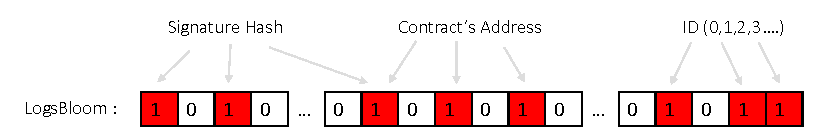
\includegraphics[width=9cm]{figs/bloom_indexed.pdf}}
        \caption{}
        \label{fig:bloom_indexed}
    \end{subfigure}
    \begin{subfigure}{\linewidth}
        \centerline{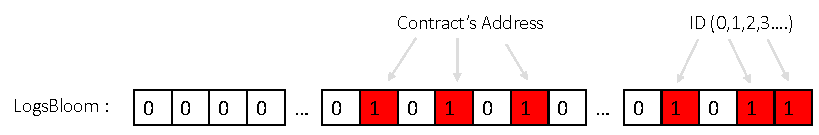
\includegraphics[width=9cm]{figs/bloom_anonymous.pdf}}
        \caption{}
        \label{fig:bloom_anonymous}
    \end{subfigure}
    \caption{Example of the bloom bits set by (a) indexed (b) anonymous indexed events.}
    \label{fig:bloom_combined}
\end{figure}

It is noteworthy that Geth uses LevelDB to manage the blockchain's data. Driven by the fact that most operating systems utilize free RAM memory for caching, we decided to assess how the system’s cache may influence the retrieval performance. In short, recently accessed LevelDB files are cached by the OS and therefore subsequent requests are served faster. So, we repeated our experiments but dropped the page cache between each run, as it is proposed in  \citep{perez_2020}, and gathered the measurements in Table~\ref{tab:retrieve_clear}. This dramatically delayed the retrieval of data from logs when the starting block was set to zero (i.e., beginning of the chain). Basically, when filtering from block zero, a lot of LevelDB files are accessed to find a specific log. The fact that these files are loaded from disk when they are not available in the system’s cache, justifies this delay. On the other hand, since the required disk accesses are greatly reduced when the search is conducted with a more recent starting point, the retrieval latency is not affected to the same extent.

\begin{table}[htbp]
\caption{Retrieval latency in Ethereum with clear cache (ms)}
\label{tab:retrieve_clear}
\resizebox{9cm}{!}{%
\begin{tabular}{@{}ccc@{}}
\toprule
 & \multicolumn{2}{c}{\textbf{Retrieval Latency}} \\ \midrule
\textbf{Storage}&\multicolumn{2}{c}{1.95}\\
\textbf{Transaction}&\multicolumn{2}{c}{3.98}\\
\midrule
\textbf{} & \textbf{fromBlock: 0} & \textbf{\begin{tabular}[c]{@{}c@{}}fromBlock: con\_creation\end{tabular}} \\ \midrule
\textbf{Non Indexed Event}&1156.90&44.78\\
\textbf{Indexed Event}&1128.71&33.54\\
\textbf{Anonymous Event}&4034.35&78.19\\
\textbf{Anonymous Indexed Event}&1289.72&38.84\\
\textbf{Unused Inexed Event}&1136.50&31.93\\
\textbf{Unused Non Indexed Event}&1154.05&39.29\\
\bottomrule
\end{tabular}%
}
\end{table}

\begin{table*}[!h]
 \centering
\caption{Overall comparison of Ethereum's data stores.}
\label{table:overall}
\begin{tabular}{@{}p{0.1\linewidth}p{0.09\linewidth} p{0.09\linewidth}p{0.09\linewidth}p{0.55\linewidth}@{}}
\toprule
 &  & \textbf{Storage Cost} & \textbf{Retrieval Latency} & \textbf{Comments} \\* \midrule
\textbf{Storage} & & Very High  & Very Low & \multirow{3}{10cm}{Viable option only when storing small data. Should host all the data that is essential for the SC's proper operation, since data stored using any of the alternative methods is not accessible within the SC. }\\\\\\* \midrule
\multirow{4}{*}{\textbf{Event-logs}} & \textbf{Non-Indexed}& Low&Moderate &\multirow{4}{10cm}{Suitable for archiving data at a low cost. Filtering specific logs is time consuming but limiting the filtering block-range and exploiting indexed parameters can accelerate the process. Thus, events should be declared according to the DApps' needs, so that %when retrieval performance matters,%
high latency is avoided.} \\
 & \textbf{Indexed} &Low&Moderate   \\
 & \textbf{Anonymous} & Low & Very High  \\
 & \textbf{Anonymous Indexed} &Low & High   \\* \midrule
\textbf{Transaction Payload} & \textbf{CA} &Very Low - Moderate& Very Low - Very High & \multirow{3}{10cm}{Least expensive method if the target is an EOA. The transaction hashes must be saved off-chain. In case of transactions to CAs, the cost and the retrieval performance are effected by the manner the SC's fallback is implemented.} \\

% The most cost-efficient method when transactions are targeted to EOAs. Transaction hashes must be saved off-chain. For transactions to CAs cost and retrieval performance are effected by the type of the event emitted in the fallback

\textbf{} & \textbf{EOA} &Very Low& Very Low \\\\* \midrule
\textbf{Unused functions parameters} & & Very Low  & Very Low - Very High  &\multirow{4}{10cm}{A useful variant of the previous method. Data is essentially stored in the transaction payload but the ABI specification is exploited, facilitating the management of all supported data types. Events can be used for tracking the transaction hashes at the expense of retrieval performance.}\\\\\\* \bottomrule
\end{tabular}%
% }
\end{table*}

To sum up, retrieving logs is time-consuming and imposes an overhead in most of the methods we proposed. However, one can make this compromise considering the cost reduction that these alternatives bring. Apart from that, if managing an external database for storing the transaction hashes is not discouraging, data could be stored in a transaction’s payload or even in unused function parameters, without emitting an event, which imposes an extra cost. By doing so, the cost as well as the retrieval time are reduced substantially.

\section{Experiments - IPFS \& SWARM}\label{sec:}
The aim of this experiment was to examine the use of IPFS and Swarm alongside Ethereum. We stored data blocks of size 4KB–16MB in these platforms and recorded the resulting identifiers in Ethereum using both SC storage and logs. The cost related to storing these identifiers in Ethereum was examined as well. 

Details about remote experiments...
\subsection{Storing data identifiers in Ethereum}\label{subsection:}
In general, the cost of recording content identifiers in Ethereum is consistent due to the constant length of the identifiers. However, in IPFS, using a CID v1 instead of CID v0, will result in higher gas consumption as it requires more storage space. CID v1 format \citep{multiformat}, which will be the default in the near future, consists of four parts

% \[\textsc <cidv1> ::= <multibase><multicodec-version><multicodec-content-type><multihash>\]

\begin{flushleft}
\centering
$\textsc <cidv1> ::= <multibase><multicodec-version><multicodec-content-type><multihash>$
\end{flushleft}

while CID v0 contains only the \(\scriptstyle <multihash>\), which is always a SHA-256 multihash \citep{multiformat}, i.e., a 34-byte hex array with the leading bytes [0x12, 0x20], used to denote the hash function and the hash digest’s size, followed by the hash digest. The rest are implicitly assumed to be (base58btc - cidv0 - dag-pb).

Below, we briefly describe three different approaches we studied and present the related cost concerning the use of SC storage and logs as a data store for the identifiers:

\begin{itemize}[topsep=0pt, itemsep=0pt]
\item{Save the CID in its original form (string).}
\item{Save just the hash digest of the multihash in a bytes32 data type.} 
\item{Save all parts of the CID separately, either in a struct or in an event with five parameters.}
\end{itemize}

In the last scenario, the struct is declared in an appropriate manner so that the version, the content-type and the multihashe’s function code and digest size are grouped together in a single slot. The hash digest occupies a separate slot. However, since a CID encoded in any multibase points to the same content, storing it is optional.

Based on Table~\ref{tab:hash_cost}, we conclude that storing only the hash digest of the CID, is the least expensive option. That is because in storage it takes up just one storage slot and also results in the shortest log byte array. However, this approach has a downside. A hash digest cannot be converted back to a CID v1 without the hash function code, multicodec, etc. Hence, this information must be stored off-chain or the DApp would be able to handle only CIDs v0.

\begin{table}[htbp]
\centering
\caption{Cost of storing data identifiers (gas)}
\label{tab:hash_cost}
\resizebox{9cm}{!}{%
\begin{tabular}{@{}lcccc@{}}
\toprule
 & \multicolumn{2}{c}{\textbf{IPFS}} & \multicolumn{2}{c}{\textbf{Swarm}} \\* \midrule
 & \textbf{CID0} & \textbf{CID1} & \textbf{Unencrypted} & \textbf{Encrypted} \\* \midrule
\textbf{Original form (logs)}&24825&24981&23262&25086\\
\textbf{Original form (storage)}&89542&89741&44141&89757\\
\textbf{Broken down CID (logs)}&25883&25931&-&-\\
% Remix: CID0 26575 CID1 26635
\textbf{Broken down CID (storage)}&48682&68630&-&-\\
% Remix: CID0 49266 CID1 69226
\textbf{Hash digest (logs)}&23240&23240&-&-\\
\textbf{Hash digest (storage)}&44207&44207&-&-\\* \bottomrule
\end{tabular}%
}
\end{table}

The use of logs as a data store for the identifiers leads to higher retrieval latency but, be that as it may, it’s definitely a more affordable option. Actually, one would prefer to log the CID in its original form, rather than declaring an event with five parameters to hold the CID’s individual parts. The latter is more expensive since the parameters need to be ABI encoded, taking up more bytes than the complete CID. On top of that, the CID has to be reassembled to its original form.

In all the test cases we examined, the CIDs v1 were generated using the SHA-256 hash function (default option). Hash functions that produce a shorter or same-sized hash digest would result in similar gas consumption whereas hash functions like SHA-512 would increase the cost, since additional storage slots or longer log arrays would be necessary to store them.

As discussed in Section~\ref{subsec:distributed}, when it comes to Swarm, the identifiers’ representation is fairly simple. For unencrypted content 32 bytes suffice, otherwise 64 bytes are required. Thus, gas consumption in Swarm’s case is straightforward. A developer, based on the above table can choose the appropriate method.
\subsection{Local Upload and retrieval performance - IPFS \& SWARM}\label{subsection:}
The measurements presented in Fig.~\ref{fig: ipfs_swarm_upload}, indicate that uploading data up to 256KB in Swarm is quite fast. Above this threshold, performance deteriorates substantially. We must consider that data are split into chunks which are hashed and organized in a Binary Merkle Tree. Obviously, the number of calculations included in this process is proportional to the size of the data and definitely affects the upload-time.

IPFS behaves similarly, except that the size of the data has smaller impact on its performance. This mostly stems from the fact that chunk’s default size (256KB) in IPFS is 64 times the size of a Swarm chunk (4KB), rendering the process of splitting the data and organizing the chunks in a Merkle-Dag faster. Accordingly, the quite stable measurements for data up to 256KB are justified, as they fit in one chunk. To substantiate this claim, we uploaded data on IPFS with the chunker option set to 4KB instead of 256KB. In all tests, the upload latency increased significantly. In fact, Swarm proved to be far more efficient in this scenario. On top of that, the different algorithms and data structures used by each platform to split, store and link data, contribute to the performance gap between them.

\begin{figure}[htbp]
\centerline{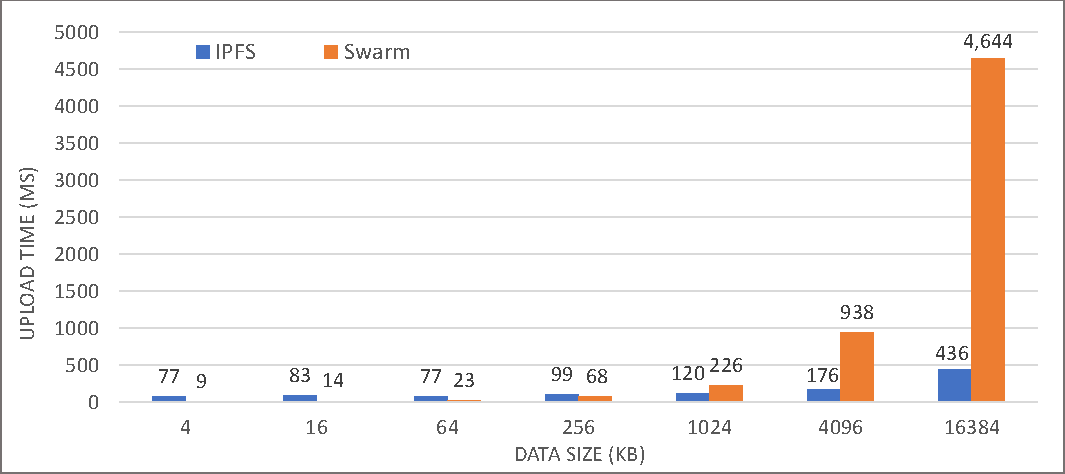
\includegraphics[width=9cm]{figs/ipfs_swarm_upload.pdf}}
\caption{IPFS-Swarm upload latency.}
\label{fig: ipfs_swarm_upload}
\end{figure}
\setlength{\belowcaptionskip}{-10pt}

As we can observe from Fig.~\ref{fig: ipfs_swarm_retrieve}, Swarm lacks in performance when it comes to retrieving data from local storage. That is due to the fact that all chunks split during the upload process must be individually fetched in order to reconstruct the original data. A large number of chunks implies a complex Merkle-Tree or Merkle-DAG. Thus, longer paths have to be resolved until each chunk is found, leading to greater retrieval time. Once again, it is clear that the chunk-size utilized within each platform’s architecture is a determining factor for their performance.

\begin{figure}[htbp]
\centerline{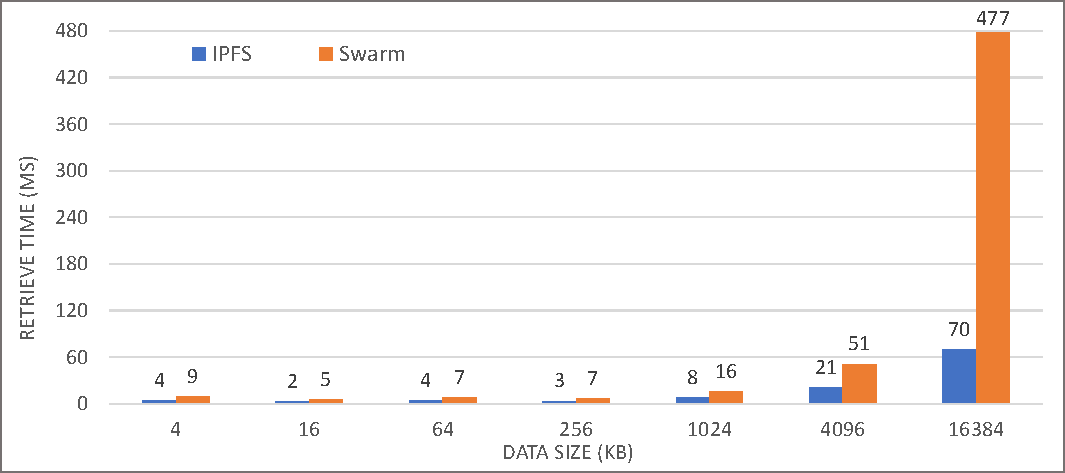
\includegraphics[width=9cm]{figs/ipfs_swarm_retrieve.pdf}}
\caption{IPFS-Swarm retrieval latency.}
\label{fig: ipfs_swarm_retrieve}
\end{figure}
\setlength{\belowcaptionskip}{-10pt}

We ought to clarify that by conducting these experiments we meant to compare the performance of IPFS and Swarm, regarding local upload and retrieval. The results are nothing but representative of how these platforms behave when exchanging data between remote nodes. Besides that, Swarm updated its networking protocol from DevP2P to LibP2P and introduced a new client, which we used during our experiments. The fact that it is in primary stage and improvements are frequently made might render our results obsolete in the near future.
\subsection{Remote Upload and retrieval performance - IPFS \& SWARM}\label{subsection:}


% TODO:

% tha mporousa isws na valw kai block kwdika apo ta smart contracts sto experimental setup i kapoio allo section gia na deiksw pws einai ta sumvolaia pou xrisimopoihsa
\cleardoublepage
% \chapter{Methods}\label{chapter:methods}
\section{Experiment}\label{sec:experiment}
\subsection{Experimental setup}\label{subsection:set-up}
\section{Data processing}\label{sec:experiment}



% \cleardoublepage
% \chapter{Results}\label{chapter:results}


% \cleardoublepage
\chapter{Discussion}\label{chapter:discussion}


\cleardoublepage
\chapter{Conclusion and Outlook}\label{chapter:Conclusion}

\cleardoublepage

% ...

% Appendix______________________________________________________________________
\appendix
\chapter{Appendix}\label{chapter:appendix}

\begin{table}[H]
\centering
\begin{small}
\caption{Accumulated measurements for experiment \textit{simple} in IPFS. The dataset consists of 1050 samples in total (including failures), with retrieval failure ratio of $\sim 4\%$ }
\label{tab:normal}
\begin{tabular}{@{}lccccccc@{}}
\toprule
Size & Mean & Median & IQR & Skewness & Min & Max & Sample Size \\ \midrule
4KB & 472.96 & 211.66 & 109.01 & 3.69 & 30.04 & 5408.44 & 140\\
16KB & 135.24 & 150.64 & 28.92 & -1.06 & 30.90 & 203.29 & 143\\
64KB & 176.44 & 175.63 & 90.05 & -0.19 & 34.75 & 382.46 & 143\\
256KB & 247.11 & 239.92 & 161.51 & 1.17 & 38.85 & 712.93 & 145\\
1MB & 514.83 & 234.93 & 202.04 & 11.63 & 52.27 & 27258.04 & 146\\
4MB & 635.02 & 431.22 & 246.71 & 2.64 & 103.36 & 3260.39 & 145\\
16MB & 1797.22 & 1306.89 & 688.50 & 2.70 & 338.36 & 9525.16 & 144\\
\bottomrule
\end{tabular}
\end{small}
\end{table}


\begin{table}[H]
\centering
\caption{Accumulated measurements for each experiment in Swarm without outliers.}
\resizebox{\textwidth}{!}{%
\begin{tabular}{@{}lcccccccc@{}}
\toprule
Experiment    & \multicolumn{7}{c}{Data Size}          & Failures (\%) \\ \midrule
& 4kb  & 16kb  & 64kb  & 256kb  & 1mb  & 4mb  & 16mb              \\ \midrule
normal & 35.91 & 207.6 & 302.56 & 475.75 & 1126.42 & 3727.21 & 9815.11 & 9 \\
no-cache  & 50.49 & 258.35 & 314.25 & 467.14 & 1206.17 & 3418.18 & 8391.32 & 9 \\
disconnect  & 52.21 & 179.63 & 344.74 & 467.44 & 1247.89 & 3507.51 & 8713.88 & 7 \\
no-cache-disconnect  & 51.54 & 152.27 & 327.29 & 441.47 & 1208.57 & 3497.87 & 8567 & 10 \\
\bottomrule
\end{tabular}
}
\end{table}


\begin{table}[H]
\centering
\begin{small}
\caption{Accumulated measurements for each experiment in IPFS without outliers.}
\begin{tabular}{@{}lcccccccc@{}}
\toprule
Experiment    & \multicolumn{7}{c}{Data Size}          & Failures (\%) \\ \midrule
& 4kb  & 16kb  & 64kb  & 256kb  & 1mb  & 4mb  & 16mb              \\ \midrule
normal & 199.88 & 154.76 & 171.33 & 194.54 & 212.07 & 402.53 & 1209.93 & 4 \\
no-cache  & 160.85 & 51.96 & 72.66 & 97.88 & 116.75 & 195.59 & 638.54 & 24 \\
disconnect  & 135.36 & 124.72 & 1168.58 & 310.82 & 1360.46 & 469.56 & 1275.26 & 37 \\
no-cache-disconnect  & 151.11 & 163.59 & 263.22 & 313.85 & 1758.96 & 759.66 & 1801.96  & 53 \\
\bottomrule
\end{tabular}
\end{small}
\end{table}



\begin{table}[H]
\centering
\begin{small}
\caption{Accumulated measurements for IPFS without outliers.}
\begin{tabular}{@{}lccccccc@{}}
\toprule
Size & Mean & Median & Skewness & Min & Max & Sample Size & Outliers \\ \midrule
4KB & 146.85 & 145.64 & 0.31 & 6.99 & 394.83 & 326 & 89\\
16KB & 113.8 & 141.63 & -0.32 & 3.13 & 243.88 & 328 & 62\\
64KB & 153.98 & 158.9 & 0.67 & 3.32 & 655.62 & 295 & 89\\
256KB & 210.55 & 174.56 & 1.4 & 38.86 & 891.33 & 318 & 82\\
1MB & 737.98 & 310.51 & 1.49 & 9.67 & 3600.76 & 391 & 19\\
4MB & 564.25 & 415.7 & 1.82 & 99.65 & 2399.45 & 363 & 49\\
16MB & 1359.79 & 1216.78 & 1.21 & 297.5 & 4592.43 & 369 & 29\\
\bottomrule
\end{tabular}
\end{small}
\end{table}

\begin{table}[H]
\centering
\begin{small}
\caption{Accumulated measurements for Swarm without outliers.}
\begin{tabular}{@{}lccccccc@{}}
\toprule
Size & Mean & Median & Skewness & Min & Max & Sample Size & Outliers \\ \midrule
4KB & 43.66 & 50.49 & 0.74 & 1.19 & 182.76 & 356 & 39\\
16KB & 218.75 & 196.73 & 0.58 & 2.66 & 662.08 & 389 & 6\\
64KB & 330.4 & 319.61 & 0 & 3.32 & 677.07 & 380 & 15\\
256KB & 483.43 & 465.3 & 0.04 & 4.69 & 978.37 & 381 & 14\\
1MB & 1276.7 & 1217.82 & 0.65 & 675.32 & 2259.57 & 378 & 22\\
4MB & 3623.02 & 3520.14 & 0.5 & 2165.56 & 5889.15 & 387 & 17\\
16MB & 9037.03 & 8914.55 & 0.46 & 5822.69 & 14261.94 & 159 & 10\\
\bottomrule
\end{tabular}
\end{small}
\end{table}






\begin{table}[H]
\centering
\begin{small}
\caption{Accumulated measurements for each experiment in IPFS without outliers (degroot-miletus-nancy).}
\begin{tabular}{@{}lcccccccc@{}}
\toprule
Experiment    & \multicolumn{7}{c}{Data Size}          & Failures (\%) \\ \midrule
& 4kb  & 16kb  & 64kb  & 256kb  & 1mb  & 4mb  & 16mb              \\ \midrule
normal & 188.38 & 149.39 & 158.54 & 167.08 & 292.41 & 461.01 & 1816.65 & 0 \\
no-cache  & 146.06 & 141.99 & 143.93 & 152.68 & 261.62 & 524.04 & 1955.46 & 3 \\
disconnect  & 189.47 & 306.23 & 1252.18 & 1281.77 & 1751.59 & 1458.82 & 3536.62 & 12 \\
no-cache-disconnect  & 198.14 & 170.18 & 1230.74 & 372.82 & 1961.7 & 2011.86 & 3162.53 & 27 \\
\bottomrule
\end{tabular}
\end{small}
\end{table}


\begin{table}[H]
\centering
\begin{small}
\caption{Accumulated measurements for experiment \textit{disconnect} in IPFS. The dataset consists of 665 samples in total (including failures), with retrieval failure ratio of $\sim 6.5\%$ }
\label{tab:disconnect}
\begin{tabular}{@{}lccccccc@{}}
\toprule
Size & Mean & Median & IQR & Skewness & Min & Max & Sample Size \\ \midrule
4KB & 899.4 & 144.2 & 1040.53 & 2.14 & 6.99 & 8551.52 & 141\\
16KB & 1234.05 & 139.67 & 1051.18 & 5.94 & 3.13 & 29803.37 & 128\\
64KB & 2417.38 & 1264.5 & 2557.39 & 3.92 & 3.32 & 29352.31 & 123\\
256KB & 1474.87 & 335.85 & 1385.74 & 6.63 & 42.83 & 30001.96 & 130\\
1MB & 1431.46 & 1360.46 & 2015.44 & 0.83 & 9.67 & 5071.64 & 136\\
4MB & 1783.34 & 494.24 & 1737.18 & 5.14 & 99.65 & 27082.3 & 139\\
16MB & 2184.65 & 1363.14 & 2050.4 & 5.38 & 297.5 & 26714.33 & 133\\
\bottomrule
\end{tabular}
\end{small}
\end{table}













\begin{table}[H]
\centering
\begin{small}
\caption{IPFS: accumulated measurements for our machine (degroot). The dataset consists of 665 samples in total (including failures), with retrieval failure ratio of $\sim 6.5\%$ }
\label{tab:degroot_ipfs}
\begin{tabular}{@{}lcccccc@{}}
\toprule
Size & Mean & Median & Skewness & Min & Max & Sample Size \\ \midrule
4KB & 1421.16 & 242.18 & 1.18 & 139.82 & 5819.67 & 88\\
16KB & 1065.02 & 170.23 & 2.54 & 128.68 & 10072.69 & 86\\
64KB & 1308.95 & 249.04 & 3.58 & 131.93 & 14766.25 & 87\\
256KB & 981.47 & 313.59 & 1.89 & 143.75 & 5293.09 & 90\\
1MB & 1249.65 & 385.42 & 1.22 & 195.49 & 5071.64 & 89\\
4MB & 1799.89 & 516.34 & 4.38 & 337.33 & 21345.4 & 93\\
16MB & 2476.33 & 1499.17 & 1.72 & 995.34 & 9461.04 & 89\\
\bottomrule
\end{tabular}
\end{small}
\end{table}

\begin{table}[H]
\centering
\begin{small}
\caption{IPFS: accumulated measurements for Lille site. The dataset consists of 665 samples in total (including failures), with retrieval failure ratio of $\sim 44\%$ }
\begin{tabular}{@{}lcccccc@{}}
\toprule
Size & Mean & Median & Skewness & Min & Max & Sample Size \\ \midrule
4KB & 556.61 & 130.76 & 5.58 & 33.68 & 10806.75 & 56\\
16KB & 199.35 & 123.73 & 4.32 & 28.48 & 2182.87 & 51\\
64KB & 485.99 & 175.87 & 2.23 & 40.17 & 3269.44 & 52\\
256KB & 491.22 & 201.17 & 2.25 & 49.33 & 3402.34 & 52\\
1MB & 1325.06 & 272.27 & 6.46 & 58.97 & 27258.05 & 55\\
4MB & 1298.11 & 464.68 & 6.03 & 108.31 & 22407.71 & 54\\
16MB & 1618.79 & 1098.98 & 2.91 & 304.16 & 9793.04 & 52\\
\bottomrule
\end{tabular}
\end{small}
\end{table}





\begin{table}[H]
\centering
\begin{small}
\caption{Swarm: accumulated measurements for our machine (degroot). The dataset consists of 458 samples in total (including failures), with retrieval failure ratio of $\sim 9\%$ }
\begin{tabular}{@{}lcccccc@{}}
\toprule
Size & Mean & Median & Skewness & Min & Max & Sample Size \\ \midrule
4KB & 125.64 & 106.78 & 1.13 & 1.19 & 375.95 & 65\\
16KB & 355.39 & 356.69 & 0.35 & 6.21 & 731.93 & 65\\
64KB & 506.36 & 455.06 & 0.8 & 6.14 & 1034.46 & 65\\
256KB & 701.1 & 659.04 & 0.52 & 10.05 & 1484.6 & 65\\
1MB & 1752.64 & 1718.43 & -0.5 & 16.36 & 2673.54 & 65\\
4MB & 4703.53 & 4606.77 & -1.05 & 39.54 & 7884.58 & 66\\
16MB & 12671.97 & 11706.08 & 0.8 & 8623.28 & 18851.85 & 25\\
\bottomrule
\end{tabular}
\end{small}
\end{table}

\begin{table}[H]
\centering
\begin{small}
\caption{Swarm: accumulated measurements for Lille site. The dataset consists of 474 samples in total (including failures), with retrieval failure ratio of $\sim 8\%$ }
\begin{tabular}{@{}lcccccc@{}}
\toprule
Size & Mean & Median & Skewness & Min & Max & Sample Size \\ \midrule
4KB & 31.59 & 31.63 & 4.54 & 2.41 & 398.32 & 67\\
16KB & 129.7 & 62.44 & 1.51 & 3.38 & 515.84 & 67\\
64KB & 262.84 & 267.23 & 0.09 & 3.72 & 588.63 & 67\\
256KB & 384.88 & 365.31 & 0.45 & 5.01 & 811.72 & 67\\
1MB & 991.81 & 976.45 & -0.61 & 10.82 & 1796.9 & 68\\
4MB & 2874.76 & 2855.04 & -1.46 & 34.05 & 4680.03 & 68\\
16MB & 8463.23 & 8544.81 & -0.14 & 5822.69 & 10991.23 & 30\\
\bottomrule
\end{tabular}
\end{small}
\end{table}



\begin{figure}[htbp]
\centerline{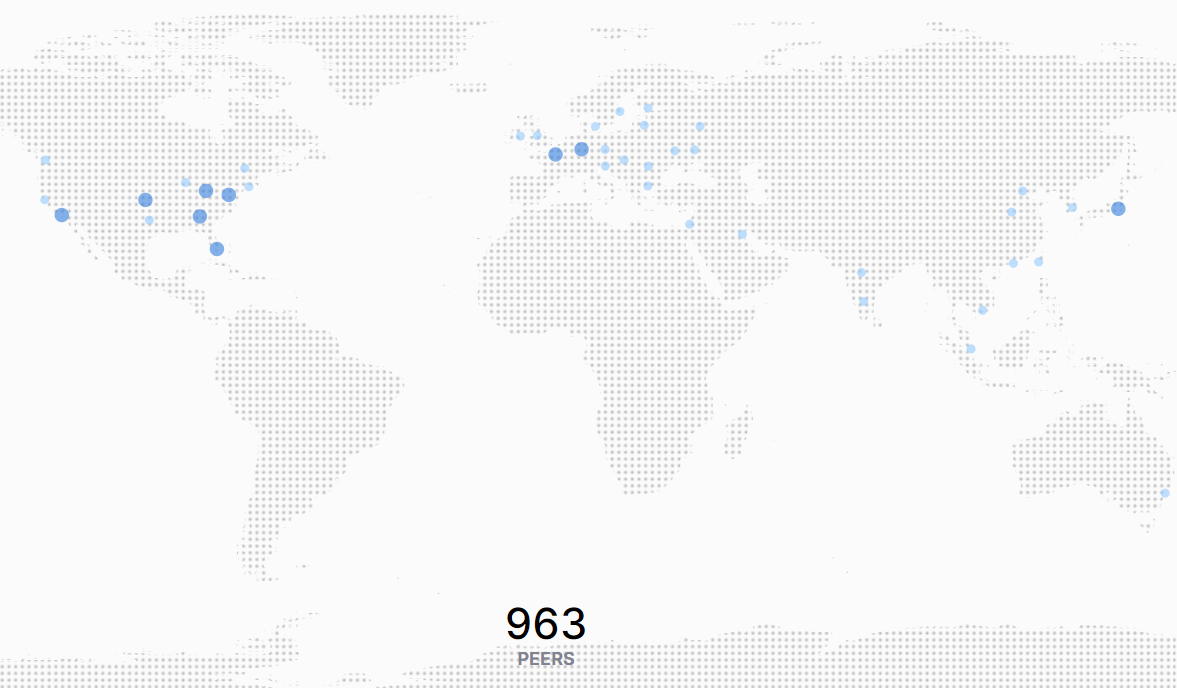
\includegraphics[width=\textwidth]{figs/ipfs_peers.png}}
\caption{EIP standardization process.}
\label{fig:ipfs_peers}
\end{figure}


% Bibliography__________________________________________________________________
% Literature (Additional references can be added to the .bib-file manually, or by using, for example, the free application JabRef). Compile in the following order: latex -bibtex -latex -latex

%\bibliographystyle{plain}
\begin{footnotesize}
\bibliographystyle{apalike}
\bibliography{references}
\end{footnotesize}

\end{document}
